\documentclass[conference]{IEEEtran}
\IEEEoverridecommandlockouts
% The preceding line is only needed to identify funding in the first footnote. If that is unneeded, please comment it out.
\usepackage{cite}
\usepackage{listings}
\usepackage{amsmath,amssymb,amsfonts}
\usepackage{algorithmic}
\usepackage{graphicx}
\usepackage{textcomp}
\usepackage{xcolor}
\def\BibTeX{{\rm B\kern-.05em{\sc i\kern-.025em b}\kern-.08em
    T\kern-.1667em\lower.7ex\hbox{E}\kern-.125emX}}
\begin{document}


\title{The Quest To Quantify Saturn's Normal-Mode Amplitudes
Using Cassini VIMS Data and Deep Learning Algorithms \\[0.5ex] \large A Project submitted in partial fulfillment for the requirement of Deep
Learning Course (CS574)}\\

\author{\IEEEauthorblockN{Victor Afigbo}
\IEEEauthorblockA{\textit{Department of Physics, University of Idaho} \\
Moscow, US \\
afig0258@vandals.uidaho.edu}\\
{Course Instructor: Prof. Min Xian, Fall Semester, 2023.}
}

\maketitle

\begin{abstract}
Planetary seismology offers a unique window into the internal dynamics of celestial bodies. In this context, we
undertake a pioneering project to predict Saturn's normal-mode amplitude values by harnessing the power of
machine learning and satellite data. Saturn, a gas giant in our solar system, exhibits complex oscillations known
as normal modes, which provide insights into its internal structure and dynamics. This project aims to leverage
deep learning techniques to predict Saturn's normal-mode amplitude values based on the Cassini VIMS data.
The study involves collecting and preprocessing of satellite data, feature engineering procedures to capture
relevant patterns, and a regression model to be trained using a dataset labeled with normal-mode amplitude
values from the theoretical linear density wave model. The deep learning model is rigorously evaluated using
various metrics, and its predictions are compared against existing theoretical results estimated using the linear
density wave model. This project at the intersection of planetary science and deep learning holds promises for
deciphering Saturn's enigmatic interior and contributing to broader advancements in planetary studies.
\end{abstract}

\begin{IEEEkeywords}
planetary seismology, deep learning, normal-mode oscillation, CASSINI VIMS, Data, regression
\end{IEEEkeywords}

\section{Introduction}
This project aims to leverage deep learning algorithms to predict normal-mode amplitudes for Saturn using data
collected during the Cassini VIMS satellite mission (2004-2017). The feasibility of this project is grounded in
the availability of a rich dataset obtained from the Cassini mission, providing valuable insights into Saturn's
normal-mode behavior.
\subsection{Data Source}
The primary data source for this project is derived from the Cassini VIMS satellite mission, spanning the period
from 2004 to 2017. The dataset includes spectral observations that have been preprocessed to extract normal-
mode amplitude values.
\subsection{Characteristics of The Proposed Data} 
Using deep learning to predict Saturn's normal-mode amplitude values from Cassini VIMS satellite data is an interesting and challenging project. The Cassini Visual and Infrared Mapping Spectrometer (VIMS) was a scientific instrument onboard NASA's Cassini spacecraft, which was part of the Cassini-Huygens mission to study Saturn and its moons. It was chiefly designed to capture data in the visual and infrared spectra, providing important information about the composition and characteristics of various objects in the Saturnian system. Some of the key characteristics of Cassini VIMS data are given below.
\subsubsection{Spectral Range}
VIMS was capable of capturing data in a wide spectral range, covering wavelengths from the ultraviolet (0.35
micrometers) to the infrared (5.1 micrometers). This broad range allowed it to observe a variety of materials and
surface features on Saturn's moons, and its rings.
\subsubsection{High Spectral Resolution} 
VIMS was characterized by high spectral resolution, enabling it to decipher differences between chemical compounds and materials based on their unique spectral signatures (properties). This made it an excellent tool for identifying surface compositions and atmospheric constituents.
\subsubsection{Imaging Capability} 
VIMS was built to capture both spectral data and images, simultaneously. It produced spectral image cubes, where each pixel contained important spectral information, thereby allowing for the
creation of detailed maps and compositional analysis.
\subsubsection{Spatial Resolution} 
VIMS had varying spatial resolutions depending on its distance from the target object within the Saturnian system. It could provide relatively high-resolution images and spectra of objects of interest, including Saturn's rings, moons, and the planet itself.
\subsubsection{Composition Analysis} 
VIMS data allowed scientists to determine the composition of surface materials, detect the presence of water ice, methane, and other chemical compounds, and study the distribution of these materials on the surfaces of Saturn's moons and rings.
\subsubsection{Atmospheric Studies} 
VIMS was used to study the atmospheres of Saturn as well as its moons, providing insights into their temperature profiles, cloud structures, and chemical compositions.
\subsubsection{Moon and Ring Observations} 
VIMS played a very crucial role in the study of Saturn's diverse moon
system, including Titan, Enceladus, and others. It helped in characterizing their surfaces and atmospheres, and
also studying their geologic processes.
\subsubsection{Ring Features} 
VIMS data contributed to the understanding of Saturn's ring system by identifying ring particle sizes, composition variations, and the presence of water ice, as well as studying ring dynamics and interactions with nearby moons.
\subsubsection{Temporal Studies} 
Over the course of the Cassini mission, VIMS collected data at various times and viewing geometries, allowing for temporal studies and changes in the Saturnian system.
\subsubsection{Data Integration} 
VIMS data were often used in conjunction with other Cassini instruments to provide a comprehensive understanding of Saturn as well as its moons, combining spectral, imaging, and other data sets.


\section{THE PROPOSED METHOD}
Cassini's VIMS instrument significantly expanded our knowledge of Saturn and its moons, providing valuable
insights into their compositions, geologic processes, and atmospheric properties. It was used extensively to
collect data on Saturn's gravitational ring perturbations, which could be used to describe its normal-mode
amplitudes. Normal modes in planetary science refer to the natural oscillations of a planet or celestial body. To
address the predictive task, we plan to employ deep learning approaches, specifically neural networks or
architectures suitable for regression tasks. Deep learning is well-suited for capturing complex patterns within
data, and we believe it can effectively model the relationship between the input features derived from Cassini
VIMS data and the corresponding normal-mode amplitudes. A detailed steps is outlined below.

\subsection{Understand the Problem}
We familiarize ourselves with Saturn's normal modes and the relevant satellite data
available. Understanding of the physics behind the normal modes and howthey might be related to the data we
have.
\subsection{Data Collection and Preprocessing}
We acquire satellite data related to Saturn's properties that could
potentially influence its normal-mode amplitudes. This chiefly includes data related to its gravitational field.
Preprocess the data to handle missing values, outliers, and to put it into a suitable format for machine learning
algorithms.
\subsection{Feature Selection (and Engineering)}
We identify the relevant features (variables) that might impact the
normal-mode amplitudes. We might need to engineer new features that capture the underlying patterns in the
data. For example, estimating the statistical measures, gradients, or ratios from the raw data.
Data Labeling: We will compare historical normal-mode amplitude data, and use it to label our dataset for
training. These historic data for amplitude values have been estimated based on existing knowledge or
simulations.
\subsection{Choose a Machine Learning Algorithm}
We select a suitable machine learning algorithm for regression tasks,
as predicting amplitude values is essentially a regression problem. Algorithms like Linear Regression, Decision
Trees, Random Forests, Support Vector Machines, or Neural Networks could be considered. We might also
experiment with ensemble methods for improved accuracy, if the need arises.
\subsection{Data Splitting}
We are going to divide our dataset into training, validation, and testing sets. The training set will be used to train the model, the validation set will help to tune hyperparameters, and the testing set will help evaluate the final model's performance.
\subsection{Model Training}
Here, we shall train our chosen machine learning algorithm using the training data. We shall
also tune the hyperparameters involved (if necessary), using the validation set to improve the model's accuracy.

\section{Theoretical Background of Our Project}
Below, in the next sections, we are going to outline the salient equations for the models used in the course of generating the required data for this research. We shall also explain all symbols where necessary. 

%.................................................................................................................
\subsection{Planetary Oscillations}\label{AA}
Considering the largest perturbations to external gravitational field \cite{article} \cite{Marley1993PlanetaryAM}\cite{Mankovich_2019}, a Saturnian oscillation mode creates a density perturbation inside the planet, which in turn creates a time-dependent Eulerian perturbation to its bulk property (the mass density corresponding
to the $lmn$ normal mode in the planet) is expressed in terms of surface spherical harmonics, $Y_{l}^{m}(\theta,\phi)$ as: 
\begin{equation}
    \rho_{lmn}^{'}(r,\theta,\phi,t) =   \rho_{lmn}^{'}(r)Y_{l}^{m}(\theta,\phi)e^{-i\sigma_{lmn}t},
\end{equation}
$\sigma_{lmn}$ is the mode oscillation frequency in the corotating frame with the planet. $r$ is the radius, $\theta$ is the colatitude, and $\phi$ is the azimuth angle respectively. The surface spherical harmonics, $Y_{l}^{m}(\theta,\phi)$, is given in terms of the associated Legendre polynomials as: 
\begin{equation}
     Y_{l}^{m}(\theta,\phi) = (-1)^{(m+|m|)/2} \sqrt{\frac{(2l+1)}{4\pi}\frac{(l-|m|)!}{(l+|m|)!}}P^{m}_{l} (\cos\theta)e^{im\phi}
\end{equation}
$\forall$  $l \in [0, \infty)$ and $m \in [-l,+l]$.

Alternatively, we can express other properties of the planetary oscillations using similar description, for example the pressure, P, or the gravitational potential, $\Phi$, in place of the density, $\rho_{lmn}^{'}(r,\theta,\phi,t)$.

In the field of seismology, we generally describe an oscillation-mode in terms of three integers, namely l, m, and n. Projecting these integers on a spherical surface, the angular degree, $l$, measures the number of circles bounding the regions of positive and negative perturbations. The oscillation's azimuthal order, $|m|$ $(m = -l, -l+1, ..., 0,..., l-1, l)$, accounts for the number of great circles passing through the polar axis that form longitudinal boundaries. The quantity, $l-|m|$, accounts for the number of latitudinal circles forming latitudinal boundaries, while $2|m|$ accounts for zero crossings in the longitudinal direction. 

Furthermore, we can visualize the planetary oscillations using few simple properties of the spherical harmonic functions. When the angular order $m$ is zero, the harmonics are called zonal and oscillate only in the latitudinal direction. When $l=|m|$ the harmononic are called sectoral and oscillate only in the longitudinal direction.  For other values of $m$ the harmonics are called tesseral and oscillate in both the longitudinal and latitudinal directions. The equivalent Cartesian wavelength for a spherical harmonic function of degree $l$ is approximately given as, $\lambda = 2\pi R/\sqrt{l(l+1)}$. R is the radius of the sphere, and this result is known as the Jeans relation \cite{https://doi.org/10.1029/2018GC007529}.

Interestingly, when $l-m$ is even, such modes are symmetric about the equator and tend to produce periodic radial gravitational perturbations in the equatorial plane, which are responsible for driving spiral density waves in the rings. But when $l-m$ is odd, such modes are anti-symmetric and are located about the equator. They produce periodic vertical perturbations in the equatorial plane, and are responsible for driving bending waves in the rings. The third integer, n, accounts for the number of radial nodes in the mode's density profile, between the center of the planet and its surface \cite{FRENCH2021114660}. When $n=0$, the mode is referred to as the fundamental-mode (f-mode). Also, when $m>0$, these modes rotate in the same direction as the planet (prograde), while $m<0$ modes rotate in opposite direction to the planet (retrograde). 

So far, the detected signals used in this work involve mostly modes with $l\geq 2$, and no $l=0$ modes, since they are not liable to generate noticeable external gravitational perturbations. A similar case holds for the dipolar f-modes ($l=1$), that are liable to generate fictitious oscillation in Saturn's center of mass \cite{FRENCH2021114660}.

From \cite{Marley1993PlanetaryAM} \cite{FRENCH2021114660}, suggestions have been made that the internal oscillations most likely to be responsible for driving density waves in the rings would be f-modes with $l=|m|$, the sectoral modes. These suggestions have been found to be true, following reported OLD-type density waves in the C-ring, with results consistent within the expectation values \cite{Hedman_2013} \cite{10.1093/mnras/stu1503}. Another side to the previous results is the table showing the values for the mass estimates from the gravitational potentials, responsible for the spiral density wave amplitudes. The table clearly shows that none of these waves were excited by one or more of Saturn's moons, this implies that, most likely, the waves detected are as a result of planetary normal-mode oscillations (remember to add a diagram here).
\begin{figure}[h] 
\centering
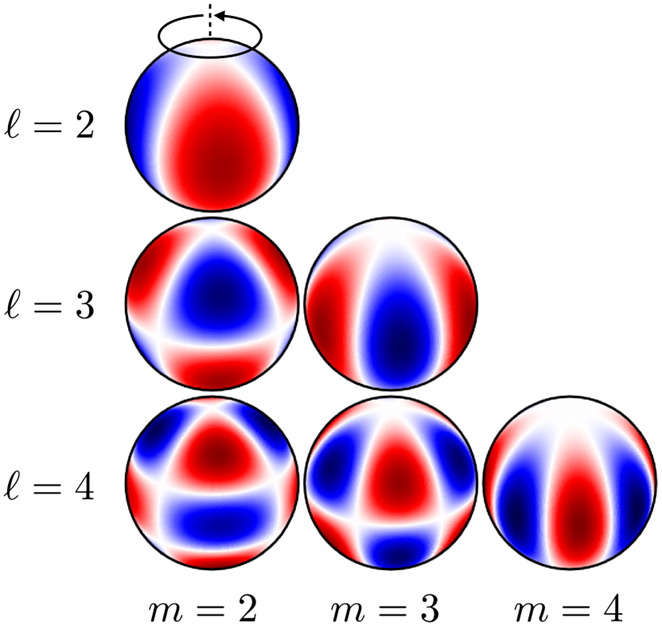
\includegraphics[width=0.5\textwidth]{mankovitch2.png}
\caption{A visual of some of the spherical harmonics relevant for Saturn ring seismology. $l$ denotes angular degree, while $m$ denotes azimuthal order \cite{Mankovich_2019}.  The color map corresponds to the magnitude of the density and gravity field perturbations, arising from oscillation. There is a downward trend of angular
degree ($l$) increase, and rightward increase in azimuthal order ($m$).} \label{fig:my_label}
\end{figure}

Understanding the aforesaid modes of oscillations help to clearly decipher the dynamics of this magnificent gas giant. Through the combination of observational data (Voyager and Cassini mostly) , theoretical models, and computer simulations, planetary scientists have been able to gain valuable insights into Saturn's internal structure, its atmospheric circulation, and the intricacies between its moons and the planet itself.
%.................................................................................................................

\subsection{Overview of Planetary Ring Seismology}

Planetary ring seismology is a field of study that uses the analysis of waves and vibrations within planetary rings to better understand their physical characteristics and formation history. By studying the way in which these waves propagate, researchers can gain insight into the density and composition of the particles within the rings, as well as the gravitational and tidal forces that influence their behavior.

On the other hand, planetary ring dynamics involves the study of the motion and behavior of particles within planetary rings. This could include the understanding of the gravitational, collisional, and electromagnetic forces that act on the particles, as well as the formation and evolution of the rings themselves.

By analyzing the distribution and behavior of the particles in a planetary ring, both areas of research can help provide researchers with more insight into the history and evolution of the planet and its moons. For example, the distribution of particles in Saturn's rings can provide information about the formation and evolution of Saturn's moon system. Also both fields could have implications for our understanding of planet formation and the evolution of planetary systems more broadly.

\subsection{Saturn’s C Ring}
Saturn's C ring is one of the most fascinating features of the sixth planet from the sun, spanning from about 74,658 km to 92,000 km from the planet's center, lying between the brighter B ring and the more diffuse D ring. The C Ring is made up of small particles ranging in size from micrometers to centimeters, and it is unique in that it has a peculiar wave-like pattern \cite{2009sfch.book..375C}\cite{Hedman_2018}\cite{Nicholson1990AnAR}. The waves across the C Ring were first observed by the Voyager spacecraft in the early 1980s. These waves are caused by gravitational interactions between the ring particles and Saturn's moons. As the moons pass by the ring, they create a gravitational disturbance that propagates through the ring in the form of a wave\cite{Hedman_2013}\cite{2014MNRAS.444.1369H}\cite{Hedman_2018}\cite{Marley1993PlanetaryAM}\cite{Nicholson1990AnAR}. These waves in the C Ring are incredibly precise, with wavelengths ranging from 30 to 180 kilometers. They are also very consistent, with the same patterns appearing year after year. The cause of this consistency is still not fully understood, but it is believed to be related to the structure of the ring particles themselves \cite{Hedman_2013}\cite{2014MNRAS.444.1369H}\cite{Hedman_2018}.

\begin{figure}[h] 
\centering
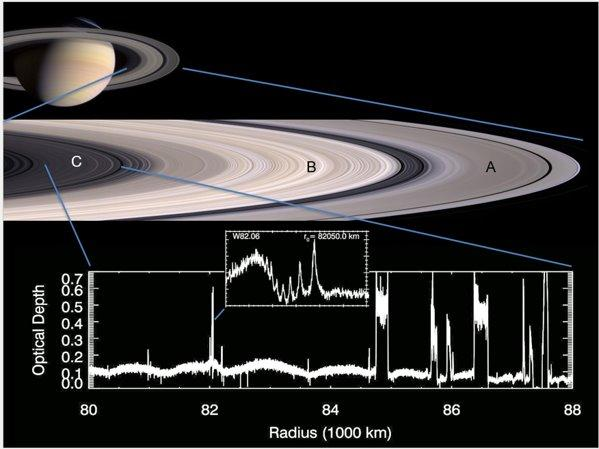
\includegraphics[width=0.47\textwidth]{Ring_Picture_Hedman_2018.jpg}
\caption{A picture of the A, B and C(Zoomed in) rings \cite{Hedman_2018}. An optical depth profile zoomed in on one of the waves (W82.06).} \label{fig:my_label}
\end{figure}

\subsection{Density Waves}
Spiral density and bending waves are well-researched and understood phenomena in the rings of Saturn, and they have provided valuable information about the surface mass density and viscosity of the main ring regions \cite{2009sfch.book..375C}\cite{Hedman_2013}\cite{2020AGUA....100142M}. The majority of these waves are caused by resonances with external satellites, especially in the A and B rings. However, another set of waves has been discovered in recent times, primarily in the C ring, which are not caused by satellites but by irregularities in Saturn's own gravitational field \cite{Hedman_2013}\cite{2014MNRAS.444.1369H}\cite{Hedman_2018}.Our focus is on studying the waves that are generated in Saturn's rings by the planetary normal modes. Specifically, we are exploring the inner C ring which has not been extensively researched before \cite{FRENCH2019599}\cite{Hedman_2013}. The waves in this area have very short wavelengths, which has posed a challenge for previous studies as they relied on precise calculations of wave phases to identify them \cite{FRENCH2019599}\cite{Hedman_2013}\cite{Hedman_2018}\cite{Tiscareno_2007}.In the next section, we aim to outline the basics of Fourier analysis and device an efficient algorithm for Fourier transformations, to use in processing Cassini's VIMS (Visual and Infrared Mapping Spectrograph) data, since other tested algorithms have resulted to an inefficient result. Thereafter, we will apply the new algorithm to our data and present the results achieved using this technique.


\subsubsection{The Theory of Spiral Density Waves: Linear Density Wave Model}
In this section, we outline the concept of spiral density waves, how it is formed across Saturn's C ring and the mathematical representation of such phenomenon.
Basically, when normal-mode oscillations take place within gaseous planets, like Saturn, they do so in terms of vibrations, and these vibrations in turn give rise to variations in density within the planet, causing disturbances to be generated within the planet, and these disturbances in turn propagate towards the exterior of Saturn. Saturn's gravitational field simply couples these disturbances to the plane of the rings, and these disturbances travel across the stretch of the ring in form of density waves, spiral density and spiral bending waves. Our main focus is on the spiral density waves since their main cause are as a result of normal mode excitation within Saturn.

For a better understanding of this work on the spiral density wave analysis, we need to outline the theory behind the algorithms used in the subsequent sections.
Here, we are utilizing the density wave model to produce anticipated wave profiles \cite{Nicholson1990AnAR}. The specific model we are using is the linear, damped model which was originally derived and elaborately introduced by Shu in 1984 \cite{article}. To provide the essential details for our project, we will give a concise explanation of the model equations as well as the model parameters. This will help us to understand the workings of the model better and enable us to use it more effectively in our project. The linear, damped model is a well-established method that has been utilized in many scientific studies to describe a variety of astronomical phenomena.

%   EDITED SECTION NOVEMBER 2023. 
%   FULL DERIVATION FOR LINEAR DENSITY WAVEMODEL

Usually, when these waves are propagated across the ring, they are displayed as fluctuations in the density of the ring's surface, which affects its optical properties. This fluctuation has an m-fold symmetry and rotates with respect to the fixed reference frame at a rate of $\Omega_{p}$. The altered surface density distribution, normalized to the background density in areas outside the waves' region, $\sigma_{0}$, is represented by the expression \cite{Nicholson1990AnAR}:

\vspace{2pt}

\begin{equation}
\Delta \sigma(r,\lambda,t) = 1 + \Re\{-iA_{L}[\pi^{-1/2}-2i\xi H(\xi)]e^{i\phi}\}e^{-(\xi /\xi_{D})^{3}}.
\end{equation}
The wave phase, $\phi$, and dimensionless distance from the resonance location, $\xi$, are clearly defined in the equations below, alongside $\xi_{D}$, which denotes the characteristic damping length of the wave. 

\vspace{2pt}

The function $H(\xi) = \pi^{-1/2}e^{-i\xi^{2}}\int_{-\infty}^{\xi}e^{i\eta^{2}}d\eta$. $H(\xi)$ includes the Standard Fresnel integral. Let $H(\xi) = \pi^{-1/2}e^{-i\xi^{2}}\gamma(\xi)$, so that the Standard Fresnel integral, $\gamma(\xi)$, is excluded from the function, $H(\xi)$. Thus we have the expression below:
\begin{equation}
    \gamma(\xi) = \int_{-\infty}^{\xi}e^{i\eta^{2}}d\eta
\end{equation}

Far into the region of wave propagation, $\xi$ is considered large and positive  \cite{Nicholson1990AnAR} \cite{1984prin.conf..513S}. Also considering the notion that the complex-Gaussian expression is exponentially convergent, we can simply separate the aforesaid integral for easy analysis resulting to the expression,
\begin{equation}
    \gamma(\xi) = \int_{-\infty}^{+ \infty}e^{i\eta^{2}}d\eta - \int_{\xi}^{\infty}e^{i\eta^{2}}d\eta = \gamma_{1} + \gamma_{2}
\end{equation}

\textbf{First Part of Integral:}
Here in this section, we are going to resolve the first part of the expanded integral for $\gamma(\xi)$, using contour integration. Let $\gamma_{1} = \int_{-\infty}^{+ \infty}e^{i\eta^{2}}d\eta$ and $\gamma_{2} = - \int_{\xi}^{\infty}e^{i\eta^{2}}d\eta$.

Considering $\gamma_{1}$, and since it is similar to the real Gaussian function, we devise a technique along the lines of Contour integration to bring it closer to the real Gaussian expression for easy analysis. Let,
\begin{equation}
    \gamma_{1} = \int_{-\infty}^{+ \infty}e^{i\eta^{2}}d\eta = 2\int_{0}^{+ \infty}e^{-(-i\eta^{2})}d\eta.
\end{equation}
Using polar coordinate expression for the arguments of $\gamma_{1}$, we have this as:
\begin{equation}
    \gamma_{1} = 2\int_{0}^{+ \infty}e^{-(e^{-i\pi/2} \eta^{2})}d\eta.
\end{equation}
We go on to factorize the previous equation and this results to, 
\begin{equation}
    \gamma_{1} = 2\int_{0}^{+ \infty}e^{-(e^{-i\pi/4} \eta)^{2}}d\eta.
\end{equation}
By substituting a variable for the exponential argument, we let $\rho = e^{-i\pi/4} \eta$ \cite{video}. Reshuffling the limits of our integral, we have: 
\begin{equation}
    \gamma_{1} = 2 e^{i\pi/4} \lim_{{R \to \infty}} \int_{0}^{Re^{-i\pi/4}} e^{-(\rho)^{2}} \, d\rho
\end{equation}

Let $\gamma_{1}^{'}$ represent the coefficient of 2 and the Euler argument in the main expression for $\gamma_{1}$, we have this as: $\gamma_{1}^{'} = \lim_{{R \to \infty}} \int_{0}^{Re^{-i\pi/4}} e^{-(\rho)^{2}} \, d\rho$, hence $\gamma_{1} = 2 e^{i\pi/4} \gamma_{1}^{'}$.

%............................................
\begin{figure}[h] 
\centering
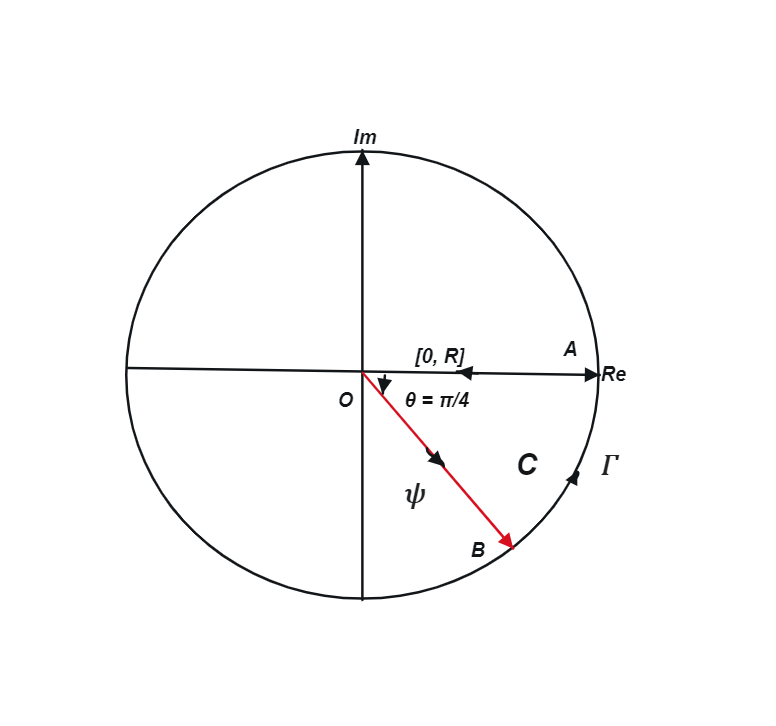
\includegraphics[width=0.7\textwidth]{COUNTOUR_INTEGRATION_DIAGRAM.png}
\caption{ Description of a pizza-shaped contour, consisting of the real (horizontal) and imaginary (vertical) axis.} \label{fig:my_label}
\end{figure}
%............................................

Considering the closed contour, as given in the diagram, for a pizza-shaped type of contour slice at an angle of $\pi/4$ radian (this angle also buttresses the asymptotic nature of $\xi$ \cite{Tiscareno_2007}), we can parametrize the previous expression and go on to evaluate the exact value of the Fresnel integral. This simply allows us to decomposed our contour integration according to the three sections present in our defined contour using complex analysis notations,
\begin{equation}
    \oint_{C} e^{-(z)^{2}} \, dz = \int_{\Psi} e^{-(z)^{2}} \, dz + \int_{\Gamma} e^{-(z)^{2}} \, dz + \int_{R}^{0} e^{-(z)^{2}} \, dz.
\end{equation}


Using Cauchy-Riemann's theorem, $\oint_{C} e^{-(z)^{2}} \, dz = 0$ (on the left hand side of the equation), since it is holomorphic inside and on $C$. Next, we consider the three sections of the given contour.

Given the conditions, $C = \left\{ z = x : 0 \leq x \leq R \right\} \cup \left\{ z : z = Re^{i\theta}, -\frac{\pi}{4} \leq \theta \leq 0 \right\} \cup \left\{ z : z = r,  0 \leq r \leq Re^{-i\frac{\pi}{4}}\right\}$, we can start with the line segment OB, $\Psi$. Here, 
\begin{equation}
    \int_{\Psi} e^{-(z)^{2}} \, dz = \int_{0}^{Re^{-i\frac{\pi}{4}}} e^{-(r)^{2}} \, dr.
\end{equation}
As $R \rightarrow \infty$, the integral along $\Psi$ assumes the format of a typical Gaussian integral, hence $\int_{0}^{\infty} e^{-(r)^{2}}\, dr = \frac{\sqrt{\pi}}{2}$.

Considering the arc BA, corresponding to the section $\Gamma$ of our contour integration,
\begin{equation}
    \int_{\Gamma} e^{-(z)^{2}} \, dz = \int_{-\frac{\pi}{4}}^{0} e^{-(z)^{2}} \, dz, \hspace{3pt} dz = iRe^{i\theta} d \theta. 
\end{equation}
By substitution we have the form for $\Gamma$ as,
\begin{equation}
    \int_{\Gamma} e^{-(z)^{2}} \, dz = \int_{-\frac{\pi}{4}}^{0} e^{-R^{2}e^{2i\theta}} iRe^{i\theta} d\theta. 
\end{equation}
Considering the absolute value of the given integral along the arc, $\Gamma$, this can be written as:
\begin{equation}
   \left| \int_{\Gamma} \right| \leq \int_{-\frac{\pi}{4}}^{0} \left|e^{-R^{2}e^{2i\theta}} iRe^{i\theta}\right| d\theta
\end{equation}
Using Euler's indentity, we reduce the expression to its real part only,
\begin{equation}
   \left| \int_{\Gamma} \right| \leq R\int_{-\frac{\pi}{4}}^{0}e^{-R^{2}\cos(2\theta)}d\theta.
\end{equation}
Intuitively, an integral like the one above with such property, vanishes as R becomes large. We are going to validate this claim analytically. A plot of $\cos(2\theta)$ $\forall \theta \in [-\frac{\pi}{4}, 0]$ simply shows that it has its minimum point at $-\frac{\pi}{4}$ and maximum point at $0$. We actually need a function within the same bound that best maximizes the $\cos(2\theta)$ within the exponential argument, to help validate our claim. An optimized function for this operation is $f(\theta) = \frac{4\theta}{\pi}+1$. This implies that, $\cos(2\theta) \geq f(\theta), \forall \theta \in [-\frac{\pi}{4}, 0]$.
Therefore, $e^{-R^{2}\cos(2\theta)} \leq e^{-R^{2}(\frac{4\theta}{\pi}+1)}$. Applying this to the previous case, 
\begin{equation}
   \left| \int_{\Gamma} \right| \leq R\int_{-\frac{\pi}{4}}^{0}e^{-R^{2}(\frac{4\theta}{\pi}+1)}d\theta = \frac{\pi}{4R}(1 - e^{-R^{2}})
\end{equation}
So we establish that, 
\begin{equation}
\lim_{{R \to \infty}} \left| \int_{\Gamma} \right| = \lim_{{R \to \infty}} \frac{\pi}{4R}(1 - e^{-R^{2}}) \leq 0.
\end{equation}

Next, we consider line segment OA, the real part of the contour. Redirecting the integral expression for that section, we have:
\begin{equation}
 \lim_{{R \to \infty}} \int_{R}^{0} e^{-(z)^{2}} \, dz = \lim_{{R \to \infty}} - \int_{0}^{R} e^{-(x)^{2}} \, dx  = -\frac{\sqrt{\pi}}{2}.
\end{equation}

Recall, $\oint_{C} e^{-(z)^{2}} \, dz = \int_{\Psi} e^{-(z)^{2}} \, dz + \int_{\Gamma} e^{-(z)^{2}} \, dz + \int_{R}^{0} e^{-(z)^{2}} \, dz.$ Using the answers to each integral, $0 = \frac{\sqrt{\pi}}{2} + 0 - \frac{\sqrt{\pi}}{2}$, which is \textbf{true}. This shows that, $\gamma_{1}^{'} = \frac{\sqrt{\pi}}{2}$ and $\gamma_{1} = \sqrt{\pi}e^{i\pi/4}$.

\vspace{3pt}

\textbf{Second Part of Integral:}
For the case of $\gamma_{1}$, we could decompose it into a standard Fresnel integral and an integral that behaves like a Fresnel function as its argument approaches infinity. Here,
\begin{equation}
\gamma_{2} = - \int_{\xi}^{\infty}e^{i\eta^{2}}d\eta = -\int_{0}^{\infty}e^{i\eta^{2}}d\eta + \int_{0}^{\xi}e^{i\eta^{2}}d\eta.
\end{equation}
Using the de Moivre's theorem, $\int_{0}^{\xi}e^{i\eta^{2}}d\eta = \int_{0}^{\xi}[cos(\eta^{2}) + isin(\eta^{2})]d\eta$. Let $C(\xi) = \int_{0}^{\xi}\cos(\eta^{2})d\eta$ and $S(\xi) =  \int_{0}^{\xi}\sin(\eta^{2})d\eta$ assume the real and imaginary parts of the asymptotic Fresnel expressions, respectively, so that $\int_{0}^{\xi}e^{i\eta^{2}}d\eta = C(\xi) + iS(\xi)$.

\vspace{5pt}

We can express the asymptotic behaviour of the aforesaid Fresnel integrals using the given forms as \cite{abramowitz1968handbook}\cite{enwiki:1181389148}\cite{wolfram-alpha-notebook}: 
\begin{equation}
    C(\xi) = \sqrt{\frac{\pi}{8}}\,\text{sgn}(\xi) + \left[1 + O\left(\xi^{-4}\right)\right]\left(\sin(\xi^2)\left(\frac{1}{2\xi}\right)\right)\right)
\end{equation}
and
\begin{equation}
   S(\xi) = \sqrt{\frac{\pi}{8}}\,\text{sgn}(\xi) - \left[1 + O\left(\xi^{-4}\right)\right]\left(\cos(\xi^2)\left(\frac{1}{2\xi}\right)\right).
\end{equation}


In the case of our model, we assume a moderate propagation of the density waves, which implies that as $\xi \rightarrow \infty$, $\mathcal{O}(\xi^{-n}) \rightarrow 0$ $\forall$ $n>1$. The moderated expression for the Fresnel integrals becomes, 
\begin{equation}
\int_{0}^{\xi}e^{i\eta^{2}}d\eta = \frac{1}{2}\left[\sqrt{\pi}e^{i\frac{\pi}{4}}\,\text{sgn}(\xi) - \frac{i}{\xi}e^{i\xi^{2}}\right].
\end{equation}
Therefore, 
\begin{equation}
\gamma_{2} = \frac{\sqrt{\pi}}{2}e^{i\frac{\pi}{4}}\left[\,\text{sgn}(\xi) - 1\right] + \frac{e^{i(\xi^{2} - \pi/2)}}{2\xi},
\end{equation}
so that $\gamma(\xi) = \frac{\sqrt{\pi}}{2}e^{i\frac{\pi}{4}}\left[\,\text{sgn}(\xi) + 1\right] + \frac{e^{i(\xi^{2} - \pi/2)}}{2\xi}$.

Now, we re-express  $H(\xi)$ as follows, 
\begin{equation}
    H(\xi) = \frac{e^{i(\frac{\pi}{4} - \xi^{2})}}{2}\left[\,\text{sgn}(\xi) + 1\right] + \frac{e^{i(-\pi/2)}}{2\xi \sqrt{\pi}}
\end{equation}

Considering the linear density wave equation, $\Delta \sigma(r,\lambda,t)$, this becomes:
\begin{equation}
\Delta \sigma(r,\lambda,t) = 1 + \Re\{A_{L}[\xi e^{i{(\phi - 3\pi/4 - \xi^{2})}}\left[\,\text{sgn}(\xi) + 1\right]]\} e^{-(\xi/\xi_{D})^{3}}
\end{equation}

Using the de Moivre's theorem as well as the real part of the linear density wave equation, this expression becomes as: 
\begin{equation}
   \Delta \sigma(r,\lambda,t) = A_{L}\xi\\e^{-\left(\frac{\xi_{*}}{\xi_{D}}\right)^3}\cos\left(\phi-\frac{3\pi}{4}-\xi^2\right)\zeta(\xi_{*})
\end{equation}

Where $\zeta(\xi_{*})$ encompases a generalized signum function, $\zeta(\xi_{*}) = [1 + \mathrm{sgn}(m)\mathrm{sgn}(\xi)]$  and $ \mathrm{sgn}(\xi) = \left\{ \begin{array}{rcl}
1 & \forall
& \xi>0 \\ 0 & \forall & \xi=0 \\ -1 & \forall & \xi<0 \\
\end{array}\right\}$.

\vspace{3pt}

Here, $\sigma(r,\lambda,t)$ is the perturbed surface density distribution of the ring section, $r$ is the distance (in kilometers) away from the center of the planet, $\lambda$ and $t$ are the longitude and time of observation, respectively. $A_{L}$ is the dimensionless amplitude factor, it is dependent on the mass of the perturbing moon, inducing the wave \cite{Tiscareno_2007}. $\phi = m(\lambda_{s}(0)+\Omega_{s}t-\lambda$) is the wave phase; $\lambda_{s}(0)$ is the mean longitude of the satellite at $t=0$ and $\Omega_{s}$ is the orbital mean motion of the satellite. $\xi_{D}$ is the dimensionless damping parameter, which depicts the location at which the wave's amplitude ceases to grow and begins to decay. It is also sensitive to the viscosity of the ring \cite{Tiscareno_2007}.
From \cite{Nicholson1990AnAR} \cite{1984prin.conf..513S}, $\xi$ is a dimensionless quantity that specifies the distance from the resonant radius, $r_{L}$, and it is given as:
\begin{equation}
\xi = \left[\frac{3|m-1|\Omega_{L}^{2}r_{L}}{4\pi G \sigma_{0}}\right]^{\frac{1}{2}}\left(\frac{r-r_{L}}{r_{L}}\right), 
\end{equation}
and $\xi_{*} = \xi \mathrm{sgn}(r - r_{L})$.

\vspace{3pt}

The resonant radius, $r_{L}$, fixes the wave against translation in the radial direction \cite{Tiscareno_2007}. Similarly, the background surface density, $\sigma_{0}$, controls the rate at which the wavenumber increases with respect to the wave's distance from its resonant location \cite{Tiscareno_2007}. G is the Newtonian gravitational constant equivalent, in SI units, to 6.674 $\times 10^{-11} m^{3}kg^{-1}⋅s^{-2}$.
\textbf{Note:} $\zeta(\xi)$ is the general parameter used to account for spiral density waves with both positive and negative azimuthal orders, and such cases determine whether the sign of $\xi$ will either be positive or negative. We explain this in the wave-fitting routine.

\begin{figure}[h] 
\centering 
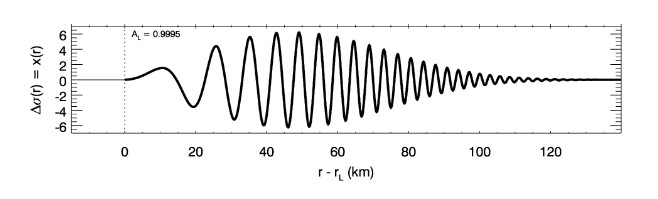
\includegraphics[width=0.5\textwidth]{Linear_Density_WM.jpg}
\caption{Synthetic density-wave radial profile generated by Equation (1) for a case of $m>0$ (prograde) \cite{Tiscareno_2007}.} \label{fig:my_label}
\end{figure}
%................................................................


\section{Methodology}
Having established the fundamental theoretical foundation for planetary oscillations and the associated effects across Saturn's (C)-ring(s), spiral density waves, our subsequent aim is to reinforce the mathematical tools employed in computing the necessary amplitudes of normal modes for Saturnian oscillations. The components of this toolbox are crucial in facilitating a precise and rigorous examination of the complex dynamics exhibited by spiral density waves, encompassing their periodic structures and frequencies.

\subsection{Wavelet Analysis}
 The method of Fourier transform provides us with valuable insights into the underlying physical properties of waves, which can be essential for understanding their behavior and predicting their future evolution. Ultimately, our application and interpretation of Fourier transform algorithms will help to shed light on the complex nature of spiral density waves and how they are excited from Saturn's interior.
 
Wavelet analysis is a method of time-frequency analysis that is scale independent and can provide more detailed information about the dominant frequencies present in a signal than traditional Fourier analysis. This is because wavelets can adapt to the local features of the signal at different scales, allowing for a more accurate representation of the signal's frequency content. In contrast, traditional Fourier analysis assumes a fixed window size, which can lead to inaccuracies in the frequency estimation of signals with non-stationary or time-varying properties. Thus, for signals with a wide range of dominant frequencies or non-stationary properties, wavelet analysis is often a more appropriate method of analysis \cite{APracticalGuidetoWaveletAnalysis}.



\subsubsection{Continous Wavelet Transform}Assuming our unprocessed wave signal is given as $x(t)$. From \cite{mertins1999signal}\cite{pereyra2012harmonic}, we use a normalized wavelet $\psi \in L^2(\mathbb{R})$, having zero average, with shifting and rescaling parameters $b$ and $a$, respectively:\begin{equation} \psi_{a,b}(t) = \frac{1}{\sqrt{|a|}} \psi\left(\frac{t-b}{a}\right)\end{equation}The Continous Wavelet Transformation derivable from our signal, $x(t)$, is given as:\begin{equation} X_{w}(a,b) = \langle x, \psi_{a,b} \rangle =\int_{-\infty}^{+\infty} x(t) \psi_{a,b}^{*}(t) \, dt\end{equation}Here, $\psi_{a,b}^{*}(t)$ is the complex conjugate of $\psi_{a,b}(t)$. We can rewrite equation 4 as: $X_{w}(a,b) = \frac{1}{\sqrt{|a|}}\int_{-\infty}^{+\infty} x(t) \bar{\psi}\left(\frac{t-b}{a}\right) dt$ and let $\tilde{X}_{w}(a,b)=\int_{-\infty}^{+\infty} x(t) \bar{\psi}\left(\frac{t-b}{a}\right) dt$. Then our new equation 4 becomes: $X_{w}(a,b)=\frac{1}{\sqrt{|a|}}\tilde{X}_{w}(a,b)$. Here, the prefactor $\frac{1}{\sqrt{|a|}}$ is introduced in order to ensure that all scaled functions with $a\in\mathbb{R}$ have the same energy \cite{mertins1999signal}\cite{Roy_2022}\cite{APracticalGuidetoWaveletAnalysis}. Note also that $b\in\mathbb{R}$.


\subsubsection{Choice of Wavelet Function}An efficient example of a normalized wavelet function that is “admissible”, has zero mean and is localized in both time and frequency space is the Morlet wavelet, comprising a plane wave modulated by a Gaussian \cite{doi:10.1146/annurev.fl.24.010192.002143}\cite{mertins1999signal}\cite{APracticalGuidetoWaveletAnalysis} and give as:\begin{equation} \psi(t)= \pi^{-1/4}e^{i\omega_{0}t}e^{-t^2/2}\end{equation}where $\omega_{0}=6$, a dimensionless frequency which satisfies the admissibility condition \cite{doi:10.1146/annurev.fl.24.010192.002143}\cite{mertins1999signal}\cite{APracticalGuidetoWaveletAnalysis}.
\begin{figure}[h]
\centering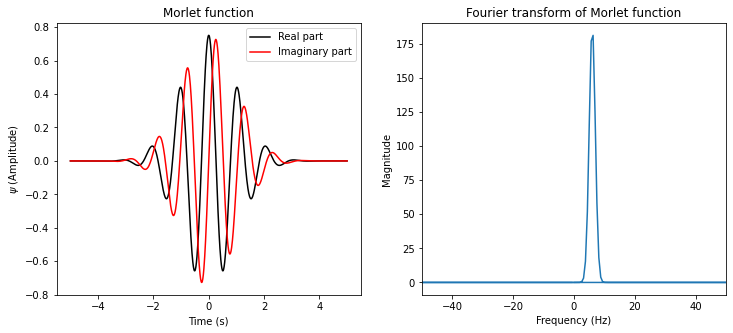
\includegraphics[width=0.5\textwidth]{Morlet_Plot_Python.png}
\caption{Morlet function in time (real and imaginary) and frequency space.} 
\label{fig:my_label}
\end{figure}
It is worthy of note that, the Morlet wavelet does not have compact support but has exponential decay. This means that the wavelet function does not go to zero outside a certain range of values, but instead decays exponentially. Regarding the differentiability of the Morlet wavelet, it is not infinitely differentiable. No wavelet with finite support can be infinitely differentiable. This is because, for a wavelet to have compact support, it must be zero outside a certain interval. However, if a function is zero outside an interval, then it cannot have nonzero derivatives of all orders.
Finally, the Morlet wavelet does not come from an MRA (multiresolution analysis). This means that the Morlet wavelet cannot be generated by a series of dilations and translations of a single wavelet function, which is a key feature of MRAs. However, the Morlet wavelet can still be used in wavelet analysis for certain applications, like in our case.


\subsubsection{Phase-Correction in Fourier Space}
After transforming our signal profile into the required wavelet, we can assume a resulting complex wavelet profile in Fourier space as \cite{Hedman_2018}, \begin{equation}    \tilde{X}_{w,i}(a,b) = \Gamma_{i}e^{i\Phi_{i}},\end{equation}where $\tilde{X}_{w,i}(a,b)$ is the complex phase-dependent wavelet transformation, $\Gamma_{i}$ is the complex amplitude, $\Phi_{i}$ is the wavelet phase which could be expressed as, $\Phi_{i} = \phi_{r}(r) + |m|(\lambda - \Omega_{p}t) + \phi_{0}$. $\phi_{r}(r)$ is the radiallly dependent portion of the wave-sphase, and for large distances from the resonant radius we can express it as \cite{1984prin.conf..513S},\begin{equation}    \phi_{r}(r) = \frac{3|m-1|M_{P}(r - r_{L})^{2}}{4\pi\sigma_{0}r^{4}_{L}}.\end{equation}All other parameters maintaining their usual meanings.   
For discrete observations of the longitude $\lambda_{i}$ and epoch time $t_{i}$, the phase parameter can be estmated using the discrete interpretation, $\phi_{i} = |m|[\lambda_{i} - \Omega_{p}t_{i}]$, given specific values of $|m|$ and $\Omega_{p}$. Given a specific wave with defined parameters, the required phase difference becomes $\Phi_{i} - \phi_{i} = \phi_{r}(r) + \phi_{0}$ for all occultations present. Now, the previous steps enables us to redefine the phase corrected wavelet as:\begin{equation}    \tilde{X}_{w,\phi,i}(a,b) = \tilde{X}_{w,i}(a,b)e^{i\Phi_{i}} = \Gamma_{i}e^{i(\Phi_{i} - \phi_{i})}.\end{equation}
Given particular signals with m and $\Omega_{p}$ values, by implication of the phase correction, there will be the same phase for all the occulation profiles present, leading to an average non-zero phase-corrected wavelet:\begin{equation}    \langle\tilde{X}_{w,\phi}(a,b)\rangle = \frac{1}{N} \sum_{i=1}^{N}\tilde{X}_{w,\phi,i}(a,b).\end{equation}


Any signal without similar phase attributes will average to zero, leaving the desired signal in the power of the average phase-corrected wavelet, expressed as,\begin{equation}    \mathcal{P}_{\phi}(r,k) = |\langle\tilde{X}_{w,\phi}(a,b)\rangle|^{2} = \left|\frac{1}{N} \sum_{i=1}^{N}\tilde{X}_{w,\phi,i}(a,b)\right|^{2}.\end{equation}On the other hand, all other signals will be captured in the average wavelet power,\begin{equation}     \bar{\mathcal{P}}(r,k) = \langle|\tilde{X}_{w,\phi}(a,b)|^{2}\rangle = \frac{1}{N} \sum_{i=1}^{N}|\tilde{X}_{w,\phi,i}(a,b)|^{2}.\end{equation}
To guage how much of the signal is consistent with the assumed m and $\Omega_{p}$, we take the ratio \cite{Hedman_2013}:  $\mathcal{T}_{\phi}(r,k) = \frac{\mathcal{P}_{\phi}(r,k)}{\bar{\mathcal{P}}(r,k)}$ $\forall$ $\mathcal{T}_{\phi}(r,k) \in (0,1)$.


\subsubsection{Wavelet Reconstruction Formula}
For proper reconstruction, we use the average phase-corrected wavelet to create a reconstructed profile with given m, and pattern speed. 

We start by assuming $x_{\phi}\in L^2(\mathbb{R})$, we can reconstruct our signal using the famous Calderon's technique \cite{Caldern1964IntermediateSA}\cite{pereyra2012harmonic}\cite{Roy_2022}\cite{APracticalGuidetoWaveletAnalysis}:
\begin{equation}
x_{\phi}(t) = \frac{1}{C_{\psi}} \int_{0}^{\infty} \int_{-\infty}^{\infty} X_{w,\phi}(a,b) \frac{1}{|a|^{1/2}} \psi\left(\frac{t-b}{a}\right) \frac{db \, da}{a^{2}},
\end{equation}
provided $\psi(t)$ satisfies Calderón's admissibility condition \cite{Caldern1964IntermediateSA}: $C_{\psi} := \int_{-\infty}^{\infty} \frac{|\tilde{\psi}(\xi)|^2}{|\xi|} d\xi < \infty$ and must have a finite energy\cite{Roy_2022}\cite{APracticalGuidetoWaveletAnalysis}: $E_{\psi} = \int_{-\infty}^{\infty} |\psi(t)|^2 dt < \infty$. Here, $\tilde\psi(\omega)$ is the Fourier transform of $\psi(t)$, $\omega = 2\pi \mathcal{\beta}$ is the angular frequency, and $C_{\psi}$ is the admissibility constant. The above condition implies that $\tilde\psi(\omega)$ approaches zero faster than $\omega$ and must not have zero frequency component, $\tilde\psi(0)=0$ \cite{Roy_2022}.


\subsubsection{Alternative Wavelet function}
Recall, $X_{w,\phi}(a,b)=\frac{1}{\sqrt{|a|}}\tilde{X}_{w,\phi}(a,b)$. By direct substitution into equation 5, we have:
\begin{equation} 
x_{\phi}(t) = \frac{1}{C_{\psi}} \int_{0}^{\infty} \int_{-\infty}^{\infty}\frac{\tilde{X}_{w,\phi}(a,b)}{|a|} \psi\left(\frac{t-b}{a}\right) \frac{db \, da}{a^{2}}.
\end{equation}



We can also choose a completely different wavelet function, Morlet's technique, like the Dirac-delta function $\delta\left(\frac{b-t}{a}\right)$, instead of the analysing wavelet \cite{doi:10.1146/annurev.fl.24.010192.002143}\cite{Roy_2022}. Here: 
\begin{equation}    x_{\phi}(t) = \frac{1}{C_{\psi}} \int_{0}^{\infty}\frac{1}{|a|} \left(\int_{-\infty}^{\infty} \tilde{X}_{w,\phi}(a,b)\delta\left(\frac{t-b}{a}\right)db\right)\frac{da}{a^2}\end{equation}

Recall for a Delta function, $\delta(-x)=\delta(x)$ and $\int_{-\infty}^{\infty}\delta(x-d)f(x) dx=f(d)$.
Using $b=ay$, and working through the double-integral, we have: $\int_{-\infty}^{\infty} \tilde{X}_{w,\phi}(a,b)\delta\left(\frac{t-b}{a}\right)db = a\tilde{X}_{w,\phi}(a,t)$.
By direct substitution into equation 5, we arrive at a simplified single integral for our wavelet reconstruction given as \cite{doi:10.1146/annurev.fl.24.010192.002143}\cite{Roy_2022}\cite{APracticalGuidetoWaveletAnalysis}:\begin{equation}     x_{\phi}(t) = \frac{1}{C_{\delta}} \int_{0}^{\infty}\frac{\tilde{X}_{w,\phi}(a,t)}{|a|}\frac{da}{a}.\end{equation}Note: $C_{\psi}=C_{\delta}$, since we reconstructed the Fourier transforms using a Dirac delta function \cite{APracticalGuidetoWaveletAnalysis}.
\subsubsection{Choice of Scale: From Dyadic to Linear Scale}Since we are working with nonorthogonal wavelet analysis, it is recommendable to use an arbitrary set of scale to build a more complete wavelet reconstruction formula for previous step above \cite{APracticalGuidetoWaveletAnalysis}. To enable us succeed in this case, we assume a variant of the dyadic scales given in \cite{pereyra2012harmonic}\cite{APracticalGuidetoWaveletAnalysis}: \begin{equation}    a_{j} =a_{0}2^{j\delta_{j}},\end{equation}where, $j=0,1,2,...,J$; $a_{0}$ is the smallest resolvable scale, assumed to be constant for our data. 



Consider the term, $\delta_{j}$, signifying the scaled range of wavelength measurement, intricately linked to the non-dimensional frequency, $\omega_{0}$. We represent this relationship as: \begin{equation}    \delta_{j} = \tilde{\epsilon}\Delta{a}.\end{equation}Here, $\delta_{j}$ encapsulates the scaled range, and its dependency on the non-dimensional frequency. This formulation precisely articulates the nuanced connection between $\delta_{j}$ and $\omega_{0}$, contingent upon the boundary condition required for an optimized result, $\tilde{\epsilon} = \sup\{\tilde{\phi} \in \mathbb{R}: 0 < \tilde{\phi} \leq \omega_0\}$, and $\Delta{a}=[a(j),a(j+1)]$, assumed to be constant for our specific signal data. 
First, to linearize the dyadic scale, we take the natural logarithm of equation (45): $\ln a_{j} = \ln a_{0} + j\delta_{j} \ln2$. Now, differentiating the previous equation with respect to the variable, $j$, simply produces the result: $\frac{da_j}{a_j} = \delta_{j} \ln2$. Note here that, $dj = (j+1)-j= 1$ for discrete case. 
Finally, we substitute the result of the latest differential equation into the equation (44), and express the total results discretely, it results to the following:\begin{equation}x_{\phi}(t) = \frac{\tilde{\epsilon}\Delta a\ln 2}{C_{\delta}} \sum_{j=0}^{J} \frac{\tilde{X}_{w,\phi}(a_{j},t)}{|a_{j}|}\end{equation}
Practically, our reconstructed time series can be taken as the sumof the real part of the wavelet transform over all scales \cite{APracticalGuidetoWaveletAnalysis}. To ensure optimal computational efficiency, we meticulously normalize and fine-tune the aforementioned reconstruction. Our final expression for achieving peak performance and accuracy becomes: \begin{equation} x_{\alpha,\phi}(t) = \tilde{\epsilon}\Delta a\lfloor \alpha \rfloor\sum_{j=0}^{J} \frac{\Re (\tilde{X}_{w,\phi}(a_{j},t))}{|a_{j}|}\end{equation}where $\alpha=\frac{ln2}{C_{\delta}\psi(0)}$, $C_{\delta}= 0.776$ \cite{APracticalGuidetoWaveletAnalysis}; $\psi(0)=\pi^{-1/4}$ \cite{APracticalGuidetoWaveletAnalysis}.$x_{\alpha,\phi}(t)$ is the final, reconstructed phase-corrected form of $x(t)$. We will use this expression in our Python computational analysis in the section below. 



\subsubsection{Sample Reconstruction}
In a bid to verify the authenticity of our customized wavelet reconstruction formula, we assume a noisy signal given by the equation:
\begin{equation}
   x(t) = 5\sin\left(\frac{2\pi t}{0.02} + 10\right) + 3\sin\left(\frac{2 \pi t}{0.05}\right)
\end{equation}
where $t &= \texttt{np.linspace(0, 1, nrx=1000)} $ in Python computations, $\Delta a=1$, $\tilde{\epsilon}=\tilde{\phi} = 6.0$ and other constants having the same value as defined previously. 

%We are going to compare our plot with that obtained using the PyWavelet Python library, below.

\begin{figure}[h]
\centering 
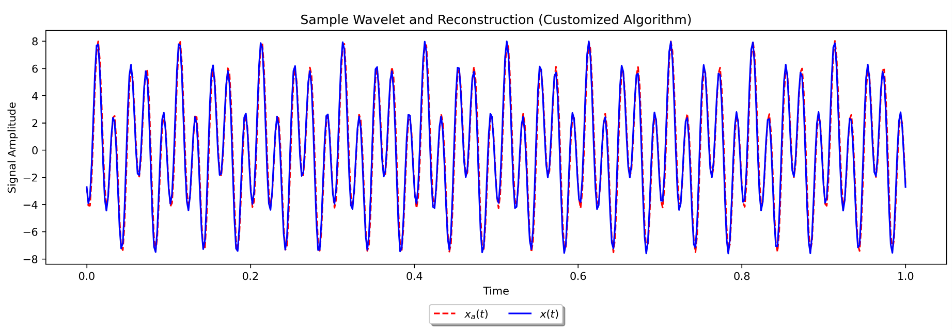
\includegraphics[width=0.5\textwidth]{Python_Wavelet_Transform_Plot_Combined.png} 
\caption{Sample Wavelet Plots (Main and Reconstructed Signals)} \label{fig:my_label}
\end{figure}

From the plot, the customized algorithm has proven to have low correction factor and a high flexibility in terms of varying the parameters for accurate results. This represents how much the wavelet transform has modified the original signal in terms of relative magnitude. Specifically, a factor greater than 1 means that the modified signal has larger amplitude than the original signal, while a factor less than 1 means that the modified signal has smaller amplitude than the original signal.

\subsection{Implementation Routine}
\subsubsection{Data acquisition}
To analyze the amplitude of spiral density waves in Saturn's C ring, we first obtained VIMS(Visual and Infrared Mapping Spectrometer) data on the C-ring structure, using Fourier analysis to break down the ring structure in terms of its individual frequency (wavelength) components. Specifically, we used data from the Cassini spacecraft, with epoch of 1o years, to obtain measurements of the density waves in the rings. The data consists of images of the rings taken by the spacecraft.
\subsubsection{Image processing}To apply Fourier transforms to the spiral density waves in Saturn's rings, we will first need to convert the set of images of the visual infrared and mapping spectrograph occultations for the ring structure, into a set of brightness values with higher values corresponding to regions of higher particle density, and vice-versa. The processed images contain information about the density waves, such as the location and shape of the waves in the images, as well as their amplitudes.
\subsubsection{Fourier transform}We will first use the Continuous Wavelet Transform (CWT) algorithm to transform the time series of the amplitude measurements into the frequency domain. This will allow us to also perform phase correction of the distorted signals, owing to blockage or distortion by the planetary body.
\subsubsection{Phase-Correction Algorithm In Fourier Space}In general, phase-correction is commonly used in signal processing to correct for phase distortions or misalignments that may have occurred during data acquisition or processing. In the context of planetary science or planetary seismology, phase correction may be used to correct for phase shifts or time delays in seismic signals caused by the propagation of seismic waves through a planetary body with a complex internal structure, like Saturn. For example, in the case of an occultation geometry, where a spacecraft passes behind a planet or moon and its signal is blocked or distorted by the planetary body, the seismic signals received by the spacecraft may be affected by the planet's internal structure, which can introduce phase shifts or time delays. By applying phase correction to the wavelet transform of the seismic signal, it may be possible to remove or mitigate some of these phase shifts or time delays, allowing for more accurate analysis and interpretation of the seismic data.
\subsubsection{Signal Reconstruction}Here, we average the resulting signals present in the whole wave occultation, after the phase-corrected has been performed. We will utilize our customized algorithm in Python computing language to recover our signals.

These plots help visualize and analyze the distribution of power and the impact of phase correction in the context of wavelet analysis. They can be valuable for identifying patterns or features in the data and understanding the effectiveness of phase correction techniques in signal processing (more to come below).
\vspace{0.5}
\textbf{Note:}The \textbf{'plt.imshow'} function is used to create these image plots. The \textbf{'vmin'} and \textbf{'vmax'} parameters control the color scale, and the \textbf{'extent'} parameter specifies the range of values for the x and y axes. The \textbf{'plt.xlabel'} and \textbf{'plt.ylabel'} functions set labels for the x and y axes of each plot.

\begin{figure}[h]
\centering
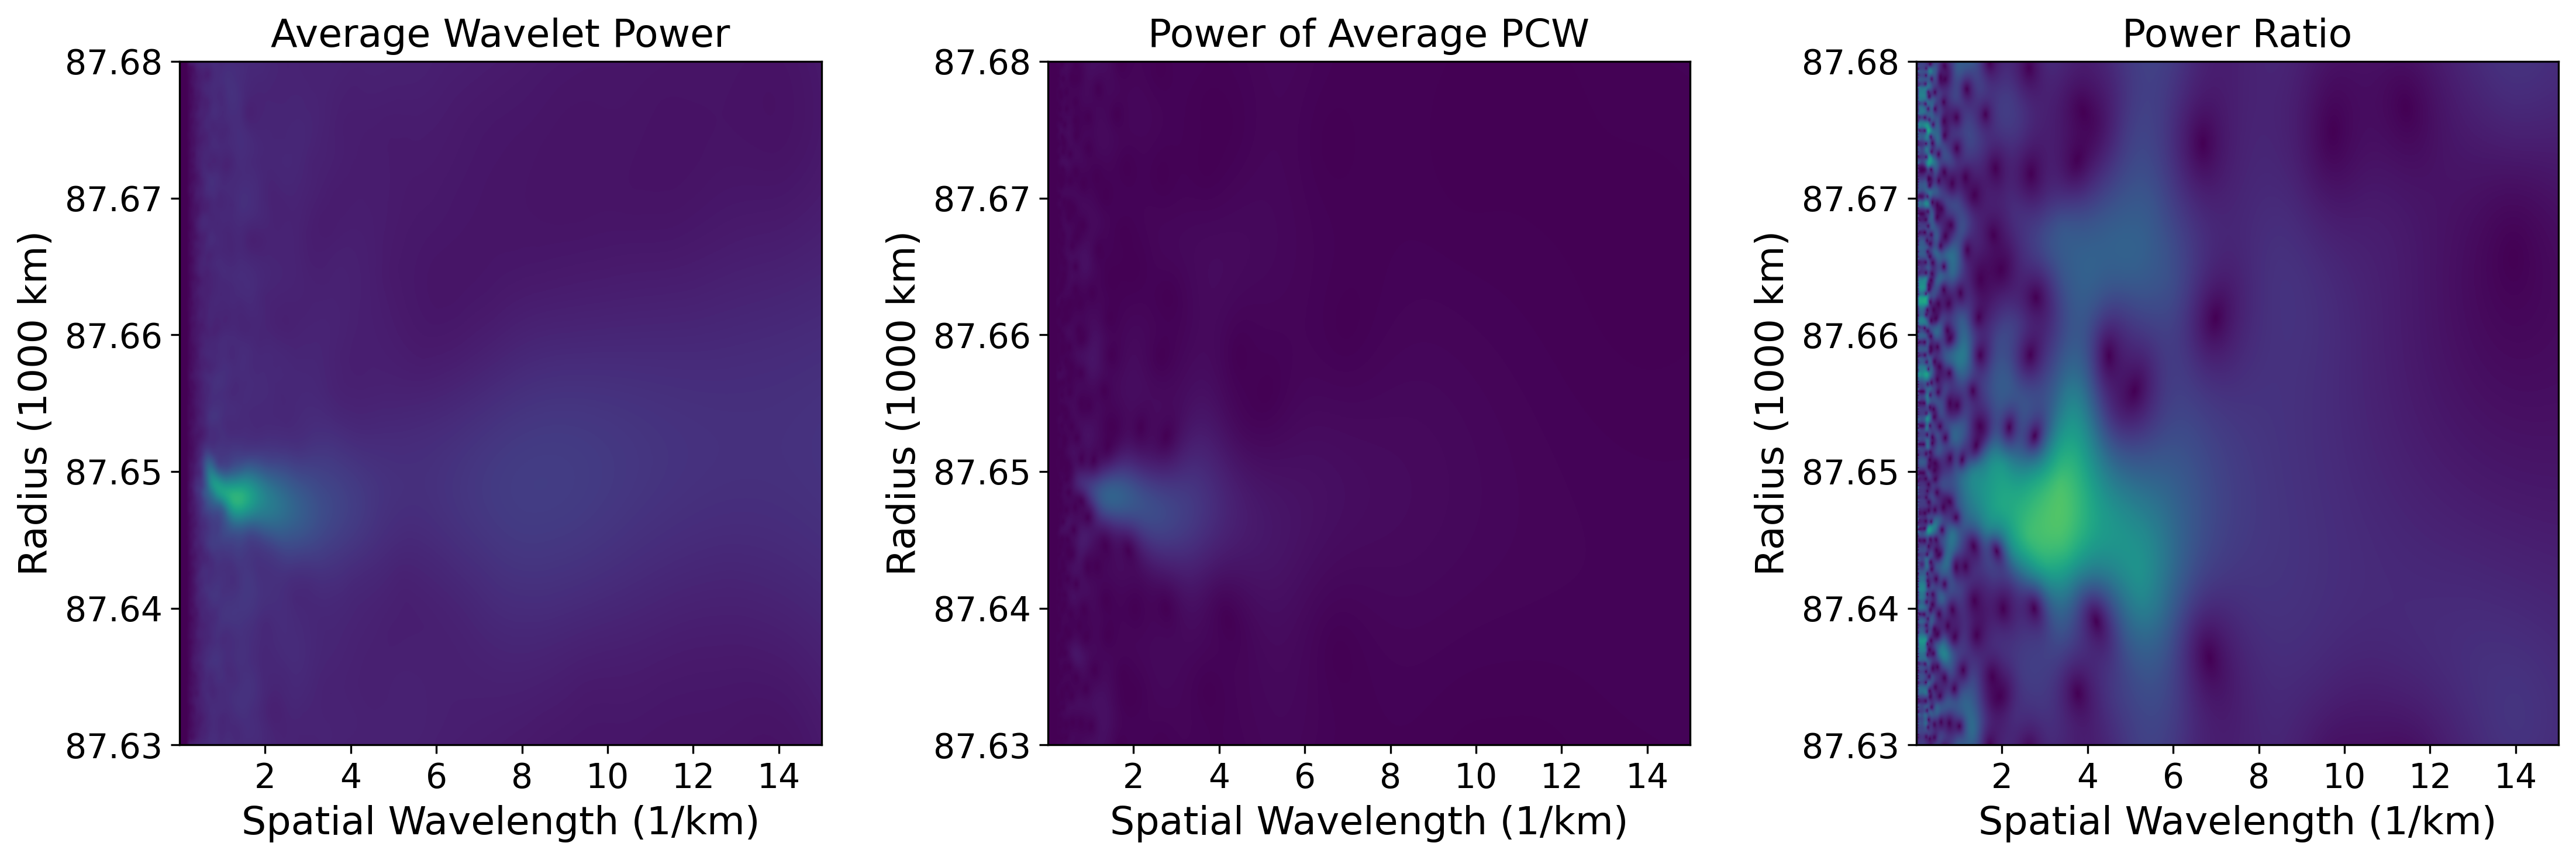
\includegraphics[width=0.5\textwidth]{power_ratio_plotw87.png}
\caption{Plots for the Power Spectrum of the Satellite resonance wavelet signal, 
\textbf{Atlas 2:1}, reveal that it falls within the radial range of 87.64 - 87.65 (in units of 1000 kilometers) and exhibits a spatial wavelength between approximately 1 and 9 (per kilometer).} 
\label{fig:my_label}
\end{figure}

A final comparison is presented in Figure 9, showcasing reconstructed occultation profiles for this specific wavelet. The top plot (orange legend) represents the average background density variations associated with the signal. The initial reconstructed average wavelet (blue legend) is a cumulative representation of the occultation profiles contained within the wavelet data. The second reconstructed wavelet plot (green legend) is the first reconstructed average wavelet, which has been normalized to the background surface density in the region of Saturn's C-ring. It is evident that the wavelet reconstruction techniques perform exceptionally well in this particular case.
\begin{figure}
\centering
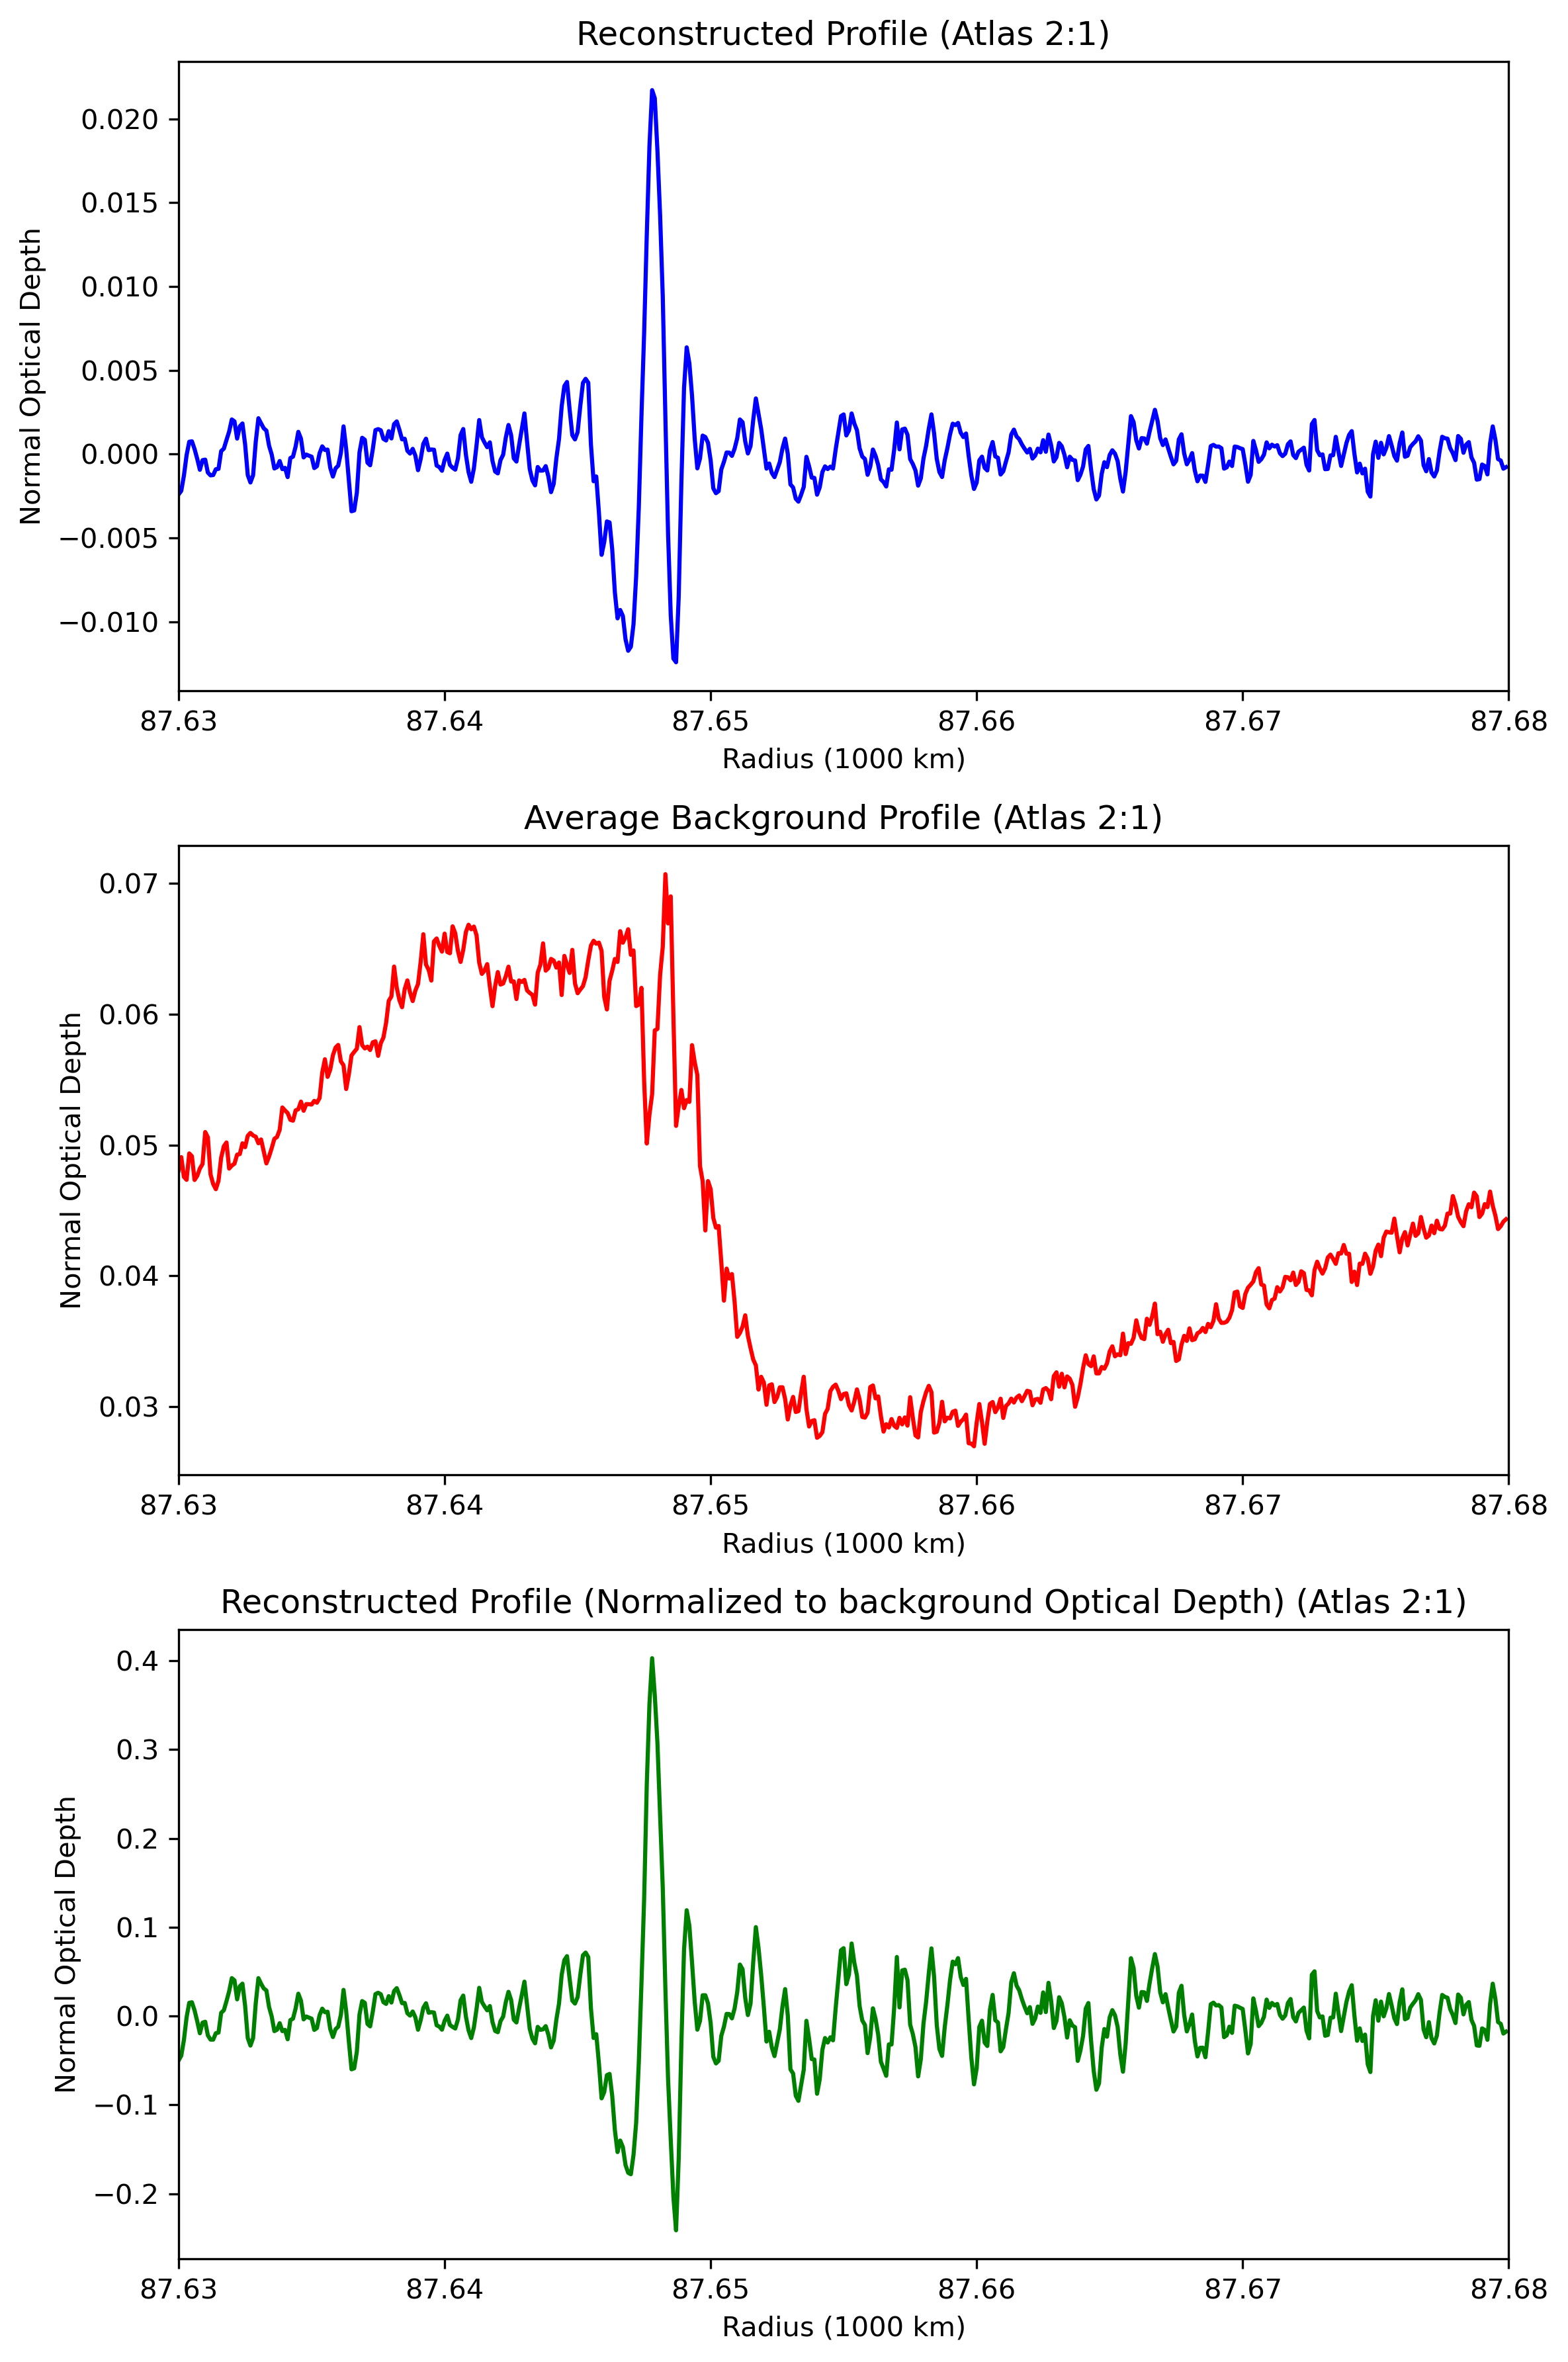
\includegraphics[width=0.5\textwidth]{combinedprofiles_atlas21.png}
\caption{A combined profiles for wavelet occultations for the Atlas 2:1 Satellite resonance.} 
\label{fig:my_label}
\end{figure}

%...............................................................................
\textbf{Final Note:}The phase-correction algorithm applies phase shifts to the wavelet transform and then computes the average phase-corrected wavelets for each pattern speed. 

\subsection{Wave-Fitting Routine}
In the process of gleaning the required information from the reconstructed signals, some pertinent parameters come to mind.
Firstly, the surface mass density, $\sigma_{0}$, which represents the mass distribution across the section of the ring, around the region of the detected wave. It is a measure of the density of matter present in the wave. The wave-fitting process can be best achieved by determining the value of $\sigma_{0}$ that best fits the observed data. We could express $\sigma_{0}$ in terms of other parameters as:
\begin{equation}
\sigma_{0} = \frac{3 |m-1| M_{P}x_{f}^{2}}{4\pi r_{L}^{4}}
\end{equation}
Here, $m$ is the azimuthal order of the wave signal. $x_{f}$ is the winding parameter from the Python Wave-fitting routine, measured in $Km$. $r_{L}$ is the resonant radius of the wave-signal.  $M_{P}$ is the mass of Saturn ($5.6846 \times 10^{26}$ Kg). \textbf{Note:} The S.I. Unit of $\sigma_{0}$ corresponds with the standard measurement in $Kgm^{-2}$.

Secondly, viscosity, $\nu$, is associated with the region of the ring where the spiral density wave is located. It measures the resistance to the flow of matter within that region of the ring. Assuming the damping phenomenon is insufficient to allow several wavecycles, we can estimate the ring section's kinematic viscosity, $\nu$, as in the case \cite{GOLDREICH1978240}\cite{1984prin.conf..513S}\cite{Tiscareno_2007}:
\begin{equation}
\nu = \frac{9}{7\Omega_{L}\xi_{D}^{3}}\left(\frac{r_{L}}{\mathcal{D}_{L}}\right)^{1/2}(2\pi G \sigma_{0})^{3/2}
\end{equation}
Where $\mathcal{D}_{L}$ = $3|m-1|\Omega_{L}^{2} + J_{2}(\frac{r_{s}}{r_{L}})^{2}[\frac{21}{2}-\frac{9}{2}|m-1|]\Omega_{L}^{2}$. The second term is only applicable as a correction factor for cases when $m \neq 1$.
Making substitutions for $\Omega_{L}$ and simplifying this equation, the viscosity becomes:
\begin{equation}
\nu = \frac{9}{7 x_{D}^{3}}(\frac{Gr_{L}^{7}}{M_{P}^{2}d_{L}})^{\frac{1}{2}}(2\pi\sigma_{0})^{\frac{3}{2}}
\end{equation}
Where $d_{L}$ = $3|m-1| + J_{2}(\frac{r_{s}}{r_{L}})^{2}[\frac{21}{2}-\frac{9}{2}|m-1|]$. $x_{D}$ is the same as $\xi_{D}$, the dimensionless damping Parameter. The new term is required for the wave-fitting routine, as we shall see in subsequent procedures. $G = 6.674 \times 10^{-11}m^{3} Kg^{-1} s^{-2}$. $r_{s} = 60330$Km (Equatorial radius for Saturn). $J_{2} = 0.01629$ (For Saturn). \textbf{Note:} The S.I. Unit of $\nu$ corresponds with measurements in $m^{2}s^{-1}$.
Thirdly, the normal-mode amplitude coefficient, $C^{'}_{lmn}$, simply represents the spherical harmonic coefficient for Saturn's gravitational field, which could be interpreted as the amplitude of the planetary oscillation responsible for exciting spiral density waves across Saturn's (C)-ring(s). Thus, when considering the case where $n=0$, the amplitude coefficient simplifies to $C^{'}_{lmn}$, which also means the modes are fundamental in nature (as described above). In subsequent sections below, we present our steps for the wave-fitting routine. Staring with the equation below, let $k_{\alpha} = \sqrt{\frac{{(2-\delta_{0,|m|})(2l+1)(l-|m|)!}}{{4\pi (l+|m|)!}}}$, so that we have:
\begin{equation}
\bar{P}_{l}^{|m|} (\mu) = k_{\alpha} P^{|m|}_{l} (\mu)
\end{equation}
We also need to rewrite equation (9) in its new (normalized) form:
\begin{equation}
\bar{\Phi}{'}(t) = \frac{GM}{r}\left\{\sum_{l=2}^{\infty}\sum_{m=-l}^{l}\left(\frac{a}{r}\right)^{l}\bar{P}_{l}^{|m|}(\mu)\bar{C}_{l|m|0}^{'}\right\}
\end{equation}
Let $(\frac{a}{r})^{l} = a_{r}^{l}$, we have:
\begin{equation}\bar{\Phi}{'}(t) = \frac{GM}{r}\left\{\sum_{l=2}^{\infty}\sum_{m=-l}^{l}a_{r}^{l}\bar{P}_{l}^{|m|}(\mu)\bar{C}_{l|m|0}^{'}\right\}
\end{equation}
By change of subject formula:
\begin{equation}
\sum_{l=2}^{\infty}\sum_{m=-l}^{l}\bar{C}_{l|m|0}^{'} =\frac{r}{GM} \sum_{l=2}^{\infty}\sum_{m=-l}^{l}\frac{\bar{\Phi}{'}(t)}{(a_{r}^{l})(\bar{P}_{l}^{|m|}(\mu))}
\end{equation}
Note:We intentionally left $\bar{\Phi}{'}(t)$ at the numerator, and after the summation symbols, because this parameter is a function of $l$ and $m$, as we shall see in the next section. 
\vspace{3}
\paragraph{Link With Wave-Fit Amplitude:}
\vspace{3}
To succinctly link the wave-fit amplitude to the gravitational potential for the planetary normal-mode oscillation, we use the expression: 
\begin{equation}
A_{\sigma_{0}}(r) = \pm \frac{\Psi_{m}^{'}}{\sqrt{\pi}G\sigma_{0} r_{L}} \sqrt{\frac{3|m - 1|M_{P}}{4 \pi \sigma_{0}r_{L}^{2}}} \frac{(r - r_{L})}{r_{L}}e^{-(|(r - r_{L})/r_{D}|)^{3}},
\end{equation}
where $\xi = \sqrt{\frac{3|m - 1|M_{P}}{4 \pi \sigma_{0}r_{L}^{2}}}\frac{(r - r_{L})}{r_{L}}$ holds the same meaning as equation (10) from \cite{Nicholson1990AnAR}. Exploring density wave signals within the context of normalized background surface density and optical depth fluctuations is essential for a comprehensive understanding of its dynamics. In this intricate analysis, it becomes imperative to articulate the amplitude of the wave in terms of its fractional form. By doing so, we delve into a nuanced examination of the intricate interplay between density variations and optical depth, unraveling deeper insights into the underlying dynamics. This approach not only enhances the precision of our observations but also paves the way for a more thorough exploration of the intricate patterns and behaviors exhibited by these density waves.

From the Python Wave-Fitting routine, the wave profile is given as a variant of equation (30):
\begin{equation}
y(x) = a(\frac{x-x_{r}}{x_{f}})e^{-\frac{(|x-x_{r}|)^{3}}{(x_{d}x_{f})^{3}}}\cos\left[\phi_{0} - \frac{3\pi}{4} - \frac{{(x-x_{r})^2}}{{x_{f}^{2}}}\right]\zeta(\frac{x-x_{r}}{x_{f}}),
\end{equation}
where, $\zeta(\frac{x-x_{r}}{x_{f}})$ is similar to $\zeta(\xi)$, but it has been customized to account for waves with differing azimuthal orders, m.
\begin{equation}
\zeta(\frac{x-x_{r}}{x_{f}}) = [1 + \mathrm{sgn}(m) \mathrm{sgn}(\frac{x-x_{r}}{x_{f}})],
\end{equation} 

Let the direct amplitude of the Wave-fit routine be given as:
\begin{equation} 
a(x) = a(\frac{x-x_{r}}{x_{f}})e^{-\frac{(|x-x_{r}|)^{3}}{(x_{d}x_{f})^{3}}}[1 + \mathrm{sgn}(m) \mathrm{sgn}(\frac{x-x_{r}}{x_{f}})]
\end{equation}
The component, $\zeta(\frac{x-x_{r}}{x_{f}})$ is only relevant in the wave-fitting procedure. Since the wave signals are usually detected at particular resonance locations, for both the retrograde ($m<0$) and prograde ($m>0$) cases, this implies that $\zeta(\frac{x-x_{r}}{x_{f}}) \rightarrow 2, \forall x \in (-\infty,+\infty)$ respectively.
Hence,
\begin{equation} 
a(x) = 2a(\frac{x-x_{r}}{x_{f}})e^{-\frac{(|x-x_{r}|)^{3}}{(x_{d}x_{f})^{3}}}
\end{equation}
Here, we treat both non-exponential terms for equations (82) and (86) on the basis that $a(x) = A_{\sigma_{0}}(r) \rightarrow r-r_{L} = x-x_{r}$:
\begin{equation}
\frac{2a}{x_{f}} = \frac{\Psi^{'}_{m}}{\sqrt{\pi} G\sigma_{0}r_{L}^{2}}\sqrt{\frac{3|m-1|M_{P}}{4\pi\sigma_{0}r_{L}^{2}}}
\end{equation}
Assuming $a = a_{fit}$, the dimensionless amplitude derived from the wave-fitting routine, we can reshuffle the equation (87) to become:
\begin{equation}
\Psi^{'}_{m} = \ 2a_{\text{fit}} \frac{\sqrt{4\pi^{2}\sigma_{0}^{3}G^{2}r_{L}^{6}}}{\sqrt{3|m-1|M_{P} x_{f}^{2}}}
\end{equation}
Recall, from \cite{Marley1993PlanetaryAM}, equation (19), we provide the link between the planetary perturbation potential and that from the density wave oscillations across the ring as:
\begin{equation}
\Psi^{'}_{m} = r \frac{d \bar{\Phi}{'}(t)}{dr} \pm 2m\bar{\Phi}{'}(t).
\end{equation}
The given equation is a first-order linear partial differential equation. It involves a partial derivative with respect to $r$ and describes a relationship between the functional perturbation potentials, $\Phi^{'}_{m}$ and $\bar{\Phi}{'}(t)$ (for the density wave across the ring surface and the planet, respectively) and $r$. The presence of the partial derivative indicates that the equation involves more than one independent variable. Resolution of the differential equation results to the general solution, say $\bar{\Phi}{'}(t) = \Phi{'}_{lm0}$:
\begin{equation}
\Psi^{'}_{m} = (2m +l+1)\Phi{'}_{lm0}.
\end{equation}
This is a standard planetary model of degree $l$ and azimuthal wavenumber, $m$. $\Phi{'}_{lm0}$ is the relevant component of the planet’s gravitational potential due to that normal-mode oscillation.
For our case, we have: $\Phi{'}_{l|m|0} = \frac{\Psi^{'}_{m}}{(2|m| + l + 1)}$. Recall, equation (68): $\sum_{l=2}^{\infty}\sum_{m=-l}^{l}\bar{C}_{l|m|0}^{'} =\frac{r}{GM} \sum_{l=2}^{\infty}\sum_{m=-l}^{l}\frac{\bar{\Phi}{'}(t)}{(a_{r}^{l})(\bar{P}_{l}^{|m|}(\mu))}$.
Let $\Phi{'}_{l|m|0} = \bar{\Phi}{'}(t)$. This is the component of the time varying gravitational potential required to estimate the normal-mode amplitudes for Saturn, considering the wave signals detected.
The new equation (68) becomes:
\begin{equation}
\sum_{l=2}^{\infty}\sum_{m=-l}^{l}\bar{C}_{l|m|0}^{'} =\frac{r}{GM} \sum_{l=2}^{\infty}\sum_{m=-l}^{l}\frac{{\Phi}^{'}_{l|m|0}}{(a_{r}^{l})(\bar{P}_{l}^{|m|}(\mu))}
\end{equation}
\textbf{Normal-mode Amplitude (N.M.A)} = \sum_{l=2}^{\infty}\sum_{m=-l}^{l}\bar{C}_{l|m|0}^{'}.


\subsubsection{Sample Wave-fitting Routine and Parameters}
To simplify the theoretical model for use in our wave-fitting routine, we use the following parameters: 
\vspace{3}
\textbf{Note:}
\vspace{3}\textbf{$a$} = Dimensionless amplitude for the density wave-fit.
\vspace{3}\textbf{$x_{d}$} = Damping parameter for the specific density wave.
\vspace{3}\textbf{$\phi_{0}$} = Initial phase value from the wave-fit routine (in radian).
\vspace{3}\textbf{$x_{r}$} = Wave-fit for the resonant radius of the wave (in Kilometer).
\vspace{3}\textbf{$x_{f}$} = Winding parameter.
\vspace{10}The attached figure illustrates the juxtaposition of two plots: one for the actual dataset from Cassini VIMS (indicated by the blue legend), and the other for the linear density wave-fitting model mentioned earlier (designated by the black legend). The vertical axis corresponds to the normalized optical depth for the section of the ring where the spiral density wave was detected by Cassini VIMS, while the horizontal axis represents the radial offset in relation to the planet's center.The necessary dimensionless parameters, including amplitude, damping, and winding, are extracted. Initially, we calculate the surface mass density using the winding parameter and subsequently derive the required viscosity. Finally, we convert the dimensionless amplitude of the spiral density wave into the necessary amplitude for the normal-mode oscillation within Saturn's interior that induced such a wave in that specific segment of Saturn's C-ring.The errors in these measurements for all wave signals are estimated through the conventional bootstrapping technique, which we will describe in the following section.

\begin{figure}[h]
\centering
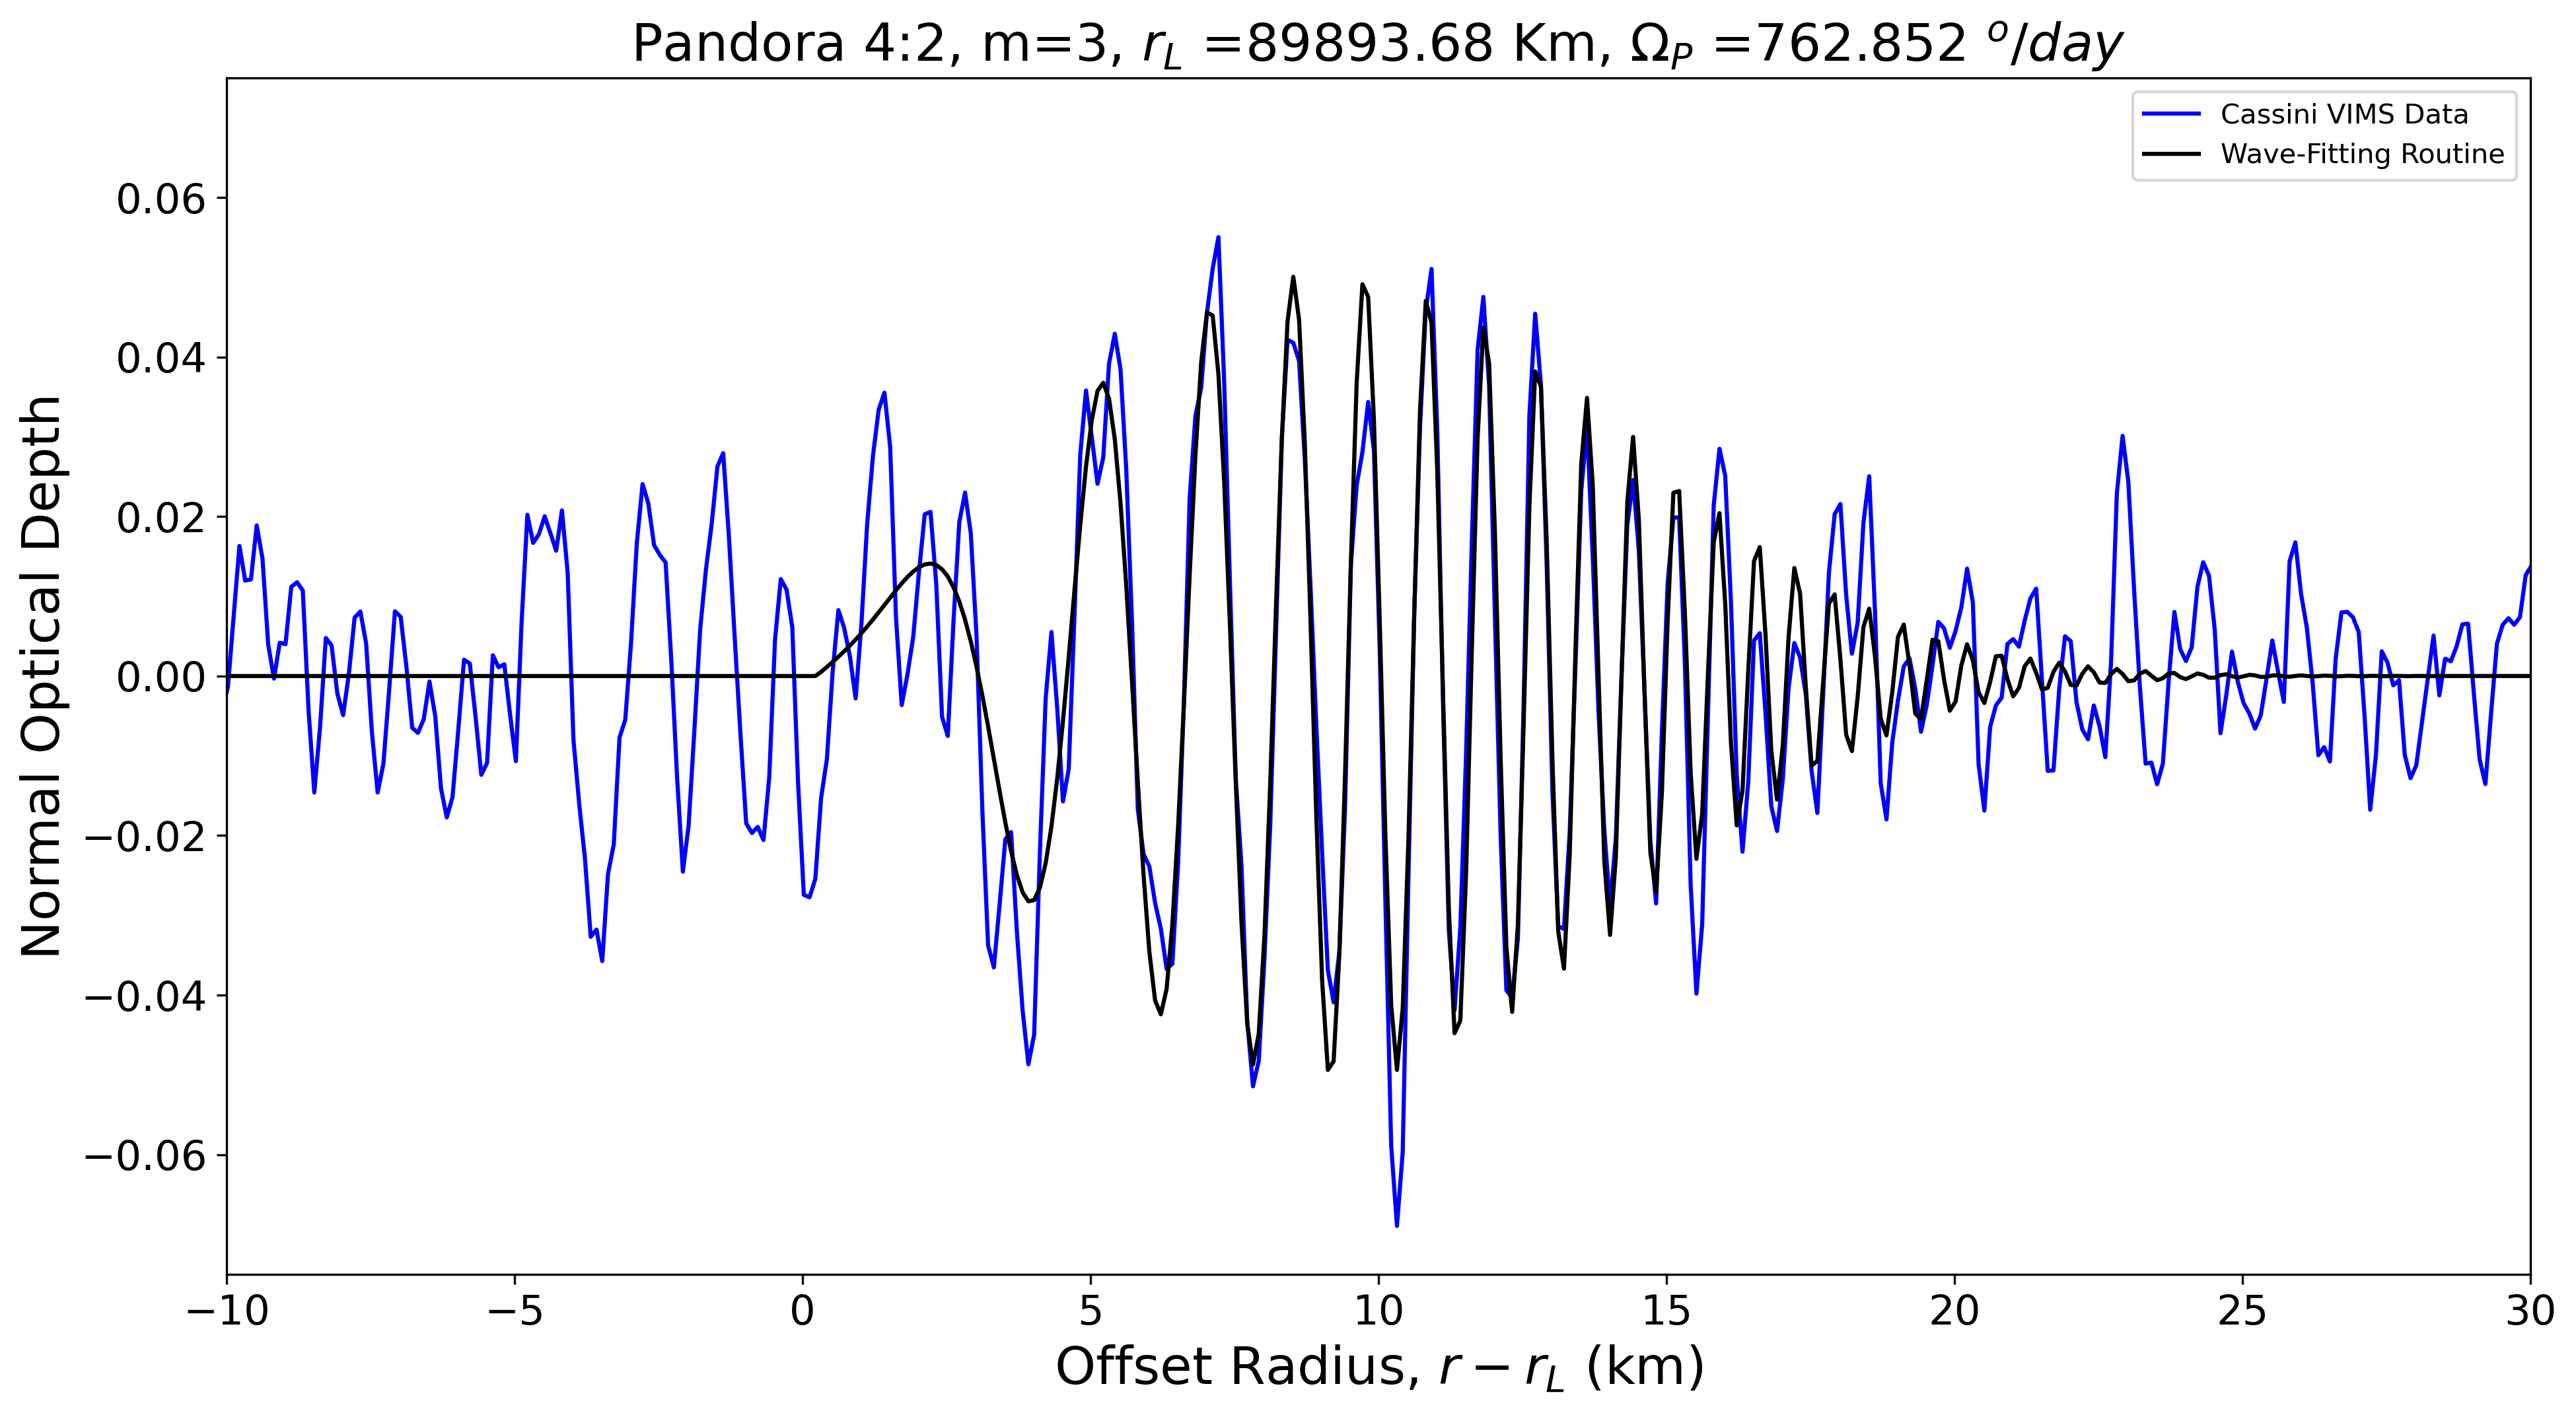
\includegraphics[width=0.5\textwidth]{pandora_42_wavefit.png}
\caption{A wave-fitting routine for the Pandora 4:2 Satellite resonance..} \label{fig:my_label}
\end{figure}


\begin{table}
\centering
\begin{tabular}{|c|c|c|}
\hline
\textbf{Nomenclature} & \textbf{Symbol} & \textbf{Value} \\
\hline
Resonance label & $m$ & 3 \\
\hline
Resonance location & $r_{L}$ & 89893.68 Km \\
\hline
Pattern speed & $\Omega_{p}$ & 762.852 $^{o}/day$ \\
\hline
Amplitude & a & 0.0074 \\
\hline
Damping Length & $x_{d}$ & 6.9140 \\
\hline
Initial Phase & $\phi_{0}$ & -3.2364 rad \\
\hline
Resonance Offset & $x_{r}$ & 0.2341 Km \\
\hline
Winding Parameter & $x_{f}$ & 1.8745 Km \\
\hline
\end{tabular}
\caption{Parameter values for wave-fitting routine for W84.64}
\end{table}

\subsection{Error Analysis by Bootstrapping}
Since each density wave profile comprises a series of occultations, there is a requirement for a precise yet efficient method to quantify uncertainties or variations in the (independent) parameters resulting from the wave-fitting routine for each wave signal. Therefore, there is a necessity for bootstrap resampling.
Bootstrap resampling is a powerful statistical technique that involves drawing multiple samples with replacement from the observed data to simulate a distribution of parameter values or estimate the uncertainty or variability in a parameter without relying on assumptions about the underlying population distribution\cite{Chernick2007BootstrapMA}\cite{davison_hinkley_1997}. By repetitively resampling the data, we can generate a range of potential parameter sets, allowing us to assess the robustness and reliability of the fitted wave profiles. That way we tend to capture the inherent variability in the data and provide a more comprehensive understanding of the uncertainties associated with the density wave parameters\cite{Efron1994AnIT}\cite{article}. This method is particularly useful for error analysis in measurements. The following steps outline the process along with relevant equations:
\paragraph{Generate Resampled Datasets}
Let $\mathbf{X} = \{x_1, x_2, \ldots, x_n\}$ represent the original dataset with $n$ measurements of a parameter (e.g., density). To perform bootstrap resampling, generate a large number of resampled datasets, denoted as $\mathbf{X}^{*}_1, \mathbf{X}^{*}_2, \ldots, \mathbf{X}^{*}_B$, each with the same size as the original dataset ($n$). Resampling is done by randomly sampling, with replacement, from the original dataset\cite{Chernick2007BootstrapMA}\cite{davison_hinkley_1997}\cite{Efron1994AnIT}\cite{article}:\begin{equation}\mathbf{X}^{*}_b = \{x^{*}_{b1}, x^{*}_{b2}, \ldots, x^{*}_{bn}\}, \quad b = 1, 2, \ldots, B\end{equation}
\paragraph{Compute the Parameter of Interest}
For each resampled dataset $\mathbf{X}^{*}_b$, where $b = 1, 2, \ldots, B$, calculate the parameter of interest, denoted as $\theta$. For example, if the interest is in the mean, the parameter estimate for the $b$th resampled dataset, denoted as $\theta^{*}_{b}$, is calculated as\cite{Chernick2007BootstrapMA}\cite{davison_hinkley_1997}\cite{Efron1994AnIT}\cite{article}:
\begin{equation}
\theta^{*}_{b} = g(\mathbf{X}^{*}_b),
\end{equation}
where $g(.)$ represents the function or statistic used to calculate the parameter estimate.
\paragraph{Calculate Variability}
After obtaining the parameter estimates $\theta^{*}_{1}, \theta^{*}_{2}, \ldots, \theta^{*}_{B}$ for all resampled datasets, analyze the distribution of these estimates to determine variability. Calculate the mean estimate ($\bar{\theta}^{*}$) and standard deviation estimate ($s^{*}$) as follows\cite{Chernick2007BootstrapMA}\cite{Efron1994AnIT}:
\begin{equation}
\bar{\theta}^{*} = \frac{1}{B}\sum_{b=1}^{B}\theta^{*}_{b},
\end{equation}

\begin{equation}
s^{*} = \sqrt{\frac{1}{B-1}\sum_{b=1}^{B}(\theta^{*}_{b} - \bar{\theta}^{*})^2}
\end{equation}
We can compute the standard error ($SE$) using the given expression\cite{Chernick2007BootstrapMA}\cite{davison_hinkley_1997}\cite{Efron1994AnIT}:
\begin{equation}
SE = \frac{s^{*}}{\sqrt{B}},
\end{equation}
and apply the aforesaid operations to our work.

\paragraph{Interpretation of the Results}
Based on the distribution of the parameter estimates, express the uncertainty in the measurement. Report the mean value and provide a confidence interval, which gives a range within which the true parameter value is likely to fall. Bootstrap resampling allows for estimating the sampling variability of a parameter without assuming a specific distribution, providing a robust method for error analysis in measurements. In essence, bootstrap resampling serves as a powerful tool for refining our analyses and ensuring that the derived parameters are not overly sensitive to specific data points, contributing to a more robust and reliable characterization of density wave profiles.
%......................................................................................

\subsection{Discussions on Model Parameters For the Wave-Fit Procedures}
Actually, there is no one-size-fits-all reason for why we chose to include the fitting parameters described above in our theoretical model. It was an essential power-play to enable us to strike a balance between the complexity of the theoretical model and the need to accurately capture the underlying behavior of the data. Our decision was guided by a combination of several factors with their succinct descriptions below.
\subsubsection{Generalization} 
The goal of modeling is often to make predictions or inferences on new, unseen data. Models with too many parameters may fit the training data extremely well but fail to generalize to new data. Reducing the number of parameters can lead to models that generalize better \cite{james2013introduction}.
\subsubsection{Quality of Data} 
High-quality, precise data can often support more complex models with more parameters. Since our data has some traces of noise, using a simpler model with fewer parameters might be more appropriate to avoid overfitting \cite{bishop2006pattern}.
\subsubsection{Overfitting} 
Overfitting is a common concern when fitting non-linear models with a large number of parameters to non-linear data. Overfitting occurs when the model captures noise and fluctuations in the data rather than the underlying trend or pattern. Reducing the number of parameters helps prevent overfitting by making the model less complex and more robust to noise \cite{bishop2006pattern}.
\subsubsection{Interpretability} 
Non-linear models with a high number of parameters can be challenging to interpret. By reducing the number of parameters, we can make the model more interpretable, as it becomes easier to understand the functional relationships between input variables and the model's predictions \cite{molnar2020interpretable}.
\subsubsection{Computational Efficiency} 
Fitting non-linear models with a large number of parameters can be computationally intensive and time-consuming. Reducing the parameter space makes the optimization problem more tractable and faster to converge using tools like SciPy \cite{nocedal2006numerical}.
\subsubsection{Stability} 
Non-linear regression can be sensitive to the initial parameter values, and models with a high number of parameters may have multiple local minima in the objective function (like degeneracies in the wave-fit parameters). Reducing the number of parameters can make the optimization process more stable and less prone to getting stuck in local optima \cite{nocedal2006numerical}.
\subsubsection{Bias-Variance Trade-off} 
Non-linear models with many parameters are prone to having high variance, which can lead to unpredictable and erratic behavior. Reducing the number of parameters can reduce model variance and improve its reliability \cite{hastie2009elements}.
\subsubsection{Data Requirements} 
Fitting complex non-linear models with numerous parameters often requires a substantial amount of data to estimate those parameters accurately. Since we are working with aliquot amount of Cassini VIMS dataset, reducing the number of parameters can help prevent overfitting and lead to more stable and trustworthy estimates.
\subsubsection{Occam's Razor} 
Ceteris paribus, this principle suggests that simpler explanations (or models) should be preferred to their complex versions. In many cases, a simpler model with fewer parameters is preferred, provided it can adequately describe the trend of dataset involved. It is easier to interpret and generalize a simple model, as opposed to a complex model \cite{Sober2015-SOBORA}.


%................................................................................
\section{Deep Learning Evaluation Plan}
The performance of our deep learning models were evaluated based on their ability to accurately predict normal-mode amplitudes. Key evaluation metrics included mean squared error (MSE), mean absolute error (MAE) and the statistical R-squared value, reflecting the models' precision and goodness of fit, since we are working on a regression problem. In details, we worked on the following below:
\subsubsection{Model Evaluation} 
We evaluated the model's performance using suitable metrics such as Mean Squared Error (MSE), Root Mean Squared Error (RMSE), Mean Absolute Error (MAE), or R-squared. The evaluation will give us an idea of how well our model predicts the normal-mode amplitudes.
\subsubsection{Iterate and Refine} 
Based on the evaluation results, we refined our model accordingly, which involved experimenting with different algorithms, tweaking features, adjusting hyperparameters, and even collecting more relevant data.
\subsubsection{Prediction} 
Once we have a trained and evaluated model, we used it to predict normal-mode amplitude values for the planetary resonance data.
\subsubsection{Interpretation} 
It was important that we interpreted the results of our machine learning model in the context of the problem. This enabled us to verify whether the predicted amplitude values were in line with existing scientific data. It might indicate a need for further refinement or a reevaluation of the underlying assumptions where necessary.

\textbf{PS:} The dataset (which exist in lump quantity, about two-dozen density wave profiles) related to this research are available on request through the planetary science research group at the Department of Physics, University of Idaho Moscow campus. For raw (unprocessed data), kindly visit the Planetary Data System (PDS) website, where Cassini mission data is archived. Use the PDS search tools to
locate the specific VIMS data sets needed, considering factors like target, time, and instrument mode.
Download the selected data files, and be prepared to process them using specialized software for analysis.
Thoroughly review accompanying documentation and metadata to understand calibration and interpretation
protocols. Conduct your research based on your objectives and remember to properly cite and acknowledge data
sources in any publications. Collaboration and available resources can also be valuable for support in working
with this data. 


\section{Experimental Results and Discussions}
\subsubsection{Dataset Preparation}
The dataset has been derived from Cassini VIMS observations during the specified timeframe. We have succeeded in extracting normal-mode amplitude values from the existing data, created a labeled dataset for training and evaluation. The required codes are given below:
\begin{lstlisting}[language=Python, caption=Data Preprocessing and Splitting, label=code:data-preprocessing]
# We define the DataFrame of Data as 'df'
# We also preprocess our data 
# (e.g., handle missing values)
df = data    #data['c_p_lm0_aav']
# We separate numeric and string columns
numeric_cols = df.select_dtypes
(include=[np.number]).columns
string_cols = df.select_dtypes
(include=[np.object]).columns

# We normalize numeric columns
scaler = MinMaxScaler()
df[numeric_cols] = 
scaler.fit_transform(df[numeric_cols])

# We encode string columns
label_encoder = LabelEncoder()
df[string_cols] = df[string_cols].
apply(lambda col: 
label_encoder.fit_transform(col.astype(str)))

# We split the data into 
# training and testing sets

train_data, test_data = 
train_test_split(df, 
test_size=0.2, random_state=42)

# We extract features (X) and target (y) 
# from the DataFrame

X_train = train_data.drop('c_p_lm0_aav', axis=1)
y_train = train_data['c_p_lm0_aav']
X_test = test_data.drop('c_p_lm0_aav', axis=1)
y_test = test_data['c_p_lm0_aav']
\end{lstlisting}


\subsubsection{Models Trained}
We have implemented and trained our deep learning models, to predict normal-mode amplitudes\cite{drori2022science}\cite{articleI}.
\begin{lstlisting}[language=Python, caption=Deep Learning Model Training, label=code:deep-learning-model]
# We build a more robust 
# and nonlinear deep learning model
model = Sequential()
model.add(Dense(128, activation='relu', 
      input_shape=(X_train.shape[1],)))
model.add(BatchNormalization())
model.add(Dropout(0.5))
model.add(Dense(64, activation='relu'))
model.add(BatchNormalization())
model.add(Dropout(0.5))
model.add(Dense(1, activation='linear'))  
# Use 'linear' for regression
\end{lstlisting}

\subsubsection{Model Parameters}
The models were trained with parameters optimized through iterative experimentation. Key parameters include, for example, learning rate, number of layers, neurons per layer, all tailored to the characteristics of the dataset\cite{drori2022science}\cite{articleI}. We also did some debugging in the general code samples, so as to make sure they produced the required results.
\begin{lstlisting}[language=Python, caption = Model Parameters, label=code:model-training]
# We compile the model with MAE as a metric
custom_optimizer = Adam(learning_rate=0.001)

model.compile(optimizer=custom_optimizer, 
loss='mean_squared_error', metrics=['mae'])

# We set up early stopping 
# to prevent overfitting
early_stopping = 
EarlyStopping(monitor='val_loss', 
patience=200, restore_best_weights=True)

# We train the more robust 
# and nonlinear model
history = model.fit(X_train, y_train, 
          epochs=1000, batch_size=32,
          validation_split=0.2, 
          callbacks=[early_stopping])
\end{lstlisting}



\subsubsection{Training and Test Accuracy}
We fine-tuned the model to exhibit promising performance during training, achieving good training and test accuracies. Initial test results indicated flawed accuracies in this case, suggesting further need to fine-tune our deep learning model in predicting Saturn's normal-mode amplitudes. Usint the codes below, along side the aforesaid parameters, we had the following table of results for the model accuracy metric:
\begin{lstlisting}[language=Python, caption=Model Evaluation Results, label=code:model-evaluation-results]
# Results obtained from model evaluation
# on the training and test set
MAE: 0.2203
MSE: 0.0729
R^{2} Score: 0.4328
\end{lstlisting}


\begin{lstlisting}[language=Python, caption=Evaluating Model Performance on Test Set, label=code:model-evaluation]
# We print MAE, MSE, 
# and R2 on the test set
y_pred = model.predict(X_test).flatten()

mae = mean_absolute_error(y_test, y_pred)
mse = mean_squared_error(y_test, y_pred)
r2 = r2_score(y_test, y_pred)

print(f'MAE:{mae:.4f}')
print(f'MSE:{mse:.4f}')
print(f'R2Score:{r2:.4f}')
\end{lstlisting}

\subsubsection{Documentation and Communication} 
Finally, we documented our methodology, choices, and results thoroughly in a \textbf{Jupyter Notebook} that will be submitted alongside this work. In general, this was a somewhat complex project that required a solid understanding of both machine learning and planetary science. Hence, we plan to collaborate with the instructor and other domain experts (in possible future outreaches, as the need arise) ensuring the model is near-perfect, and the accuracy and validity of further predictions.
\text{Note:}
In a regression problem, where it is required to predict numeric values, the concept of accuracy is typically not used. Accuracy is more relevant for classification tasks, where there are predicting categories or labels. For regression tasks, metrics like Mean Absolute Error (MAE), Mean Squared Error (MSE), and R-squared are commonly used.

\subsubsection{Plots and Discussions}
From the first plot, we have the mean absolute error and mean square error plots on the vertical axis (as well as the validation mean absolute error and validation loss) versus the number of epochs on the horizontal axis. This trend clearly shows that both class of quantities decrease, with respect to increase in the number of epochs sampled for our model. There is a clear descent around epoch number of \textbf{653}, which is clearly evident in the display section of the \textbf{Jupyter notebook} submitted. 

Additionally, the comparative plot of original and predicted normal-mode amplitudes simply shows that there were very close values for the analysed data samples. An interesting trend of relatively high correlation can be seen for index 9, 12, 21 and 25. Index 0 and 8 have relatively low correlations which could be attributable to the non-linearity of the theory that generated the datasets. 

This is an underlying issue that could be explored outside the course requirements. I plan to consult the instructor(s) involved to seek expert feedbacks on how to develop this model for optimized performance and predicted.

\begin{figure}
    \centering
    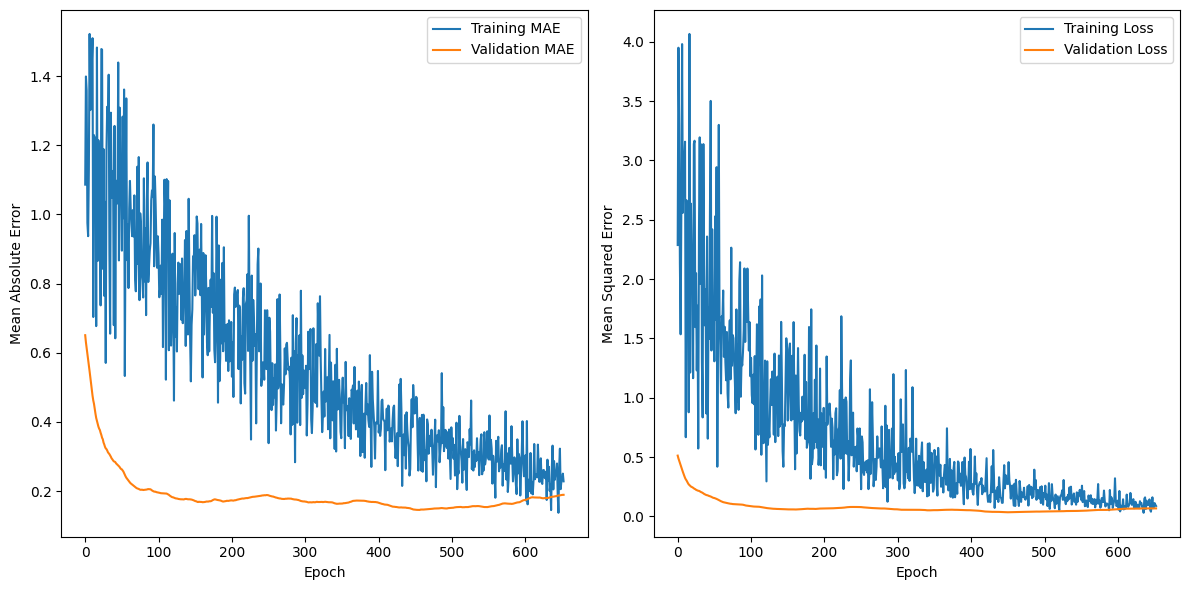
\includegraphics[width=1\linewidth]{accuracy_plots_deeplearning.png}
    \caption{Plots showing Mean Absolute Error(MAE) and Mean Square Error(MSE) versus Epoch number.}
    \label{fig:enter-label}
\end{figure}

\begin{figure}
    \centering
    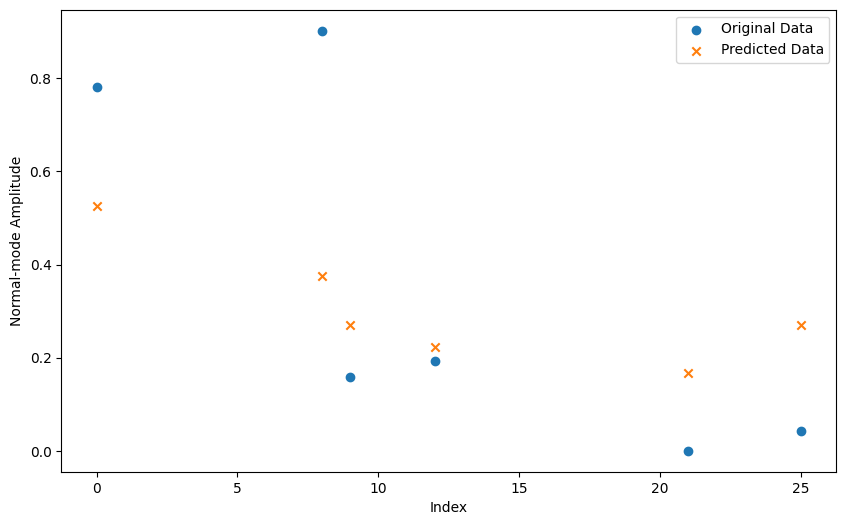
\includegraphics[width=1\linewidth]{deeplearning_prediction_plots.png}
    \caption{Plot showing the original and predicted data for Normal-mode amplitude.}
    \label{fig:enter-label}
\end{figure}

\section{Conclusion}
Evidently, we can see that the predicted normal-mode amplitude differed by around atmost 30 percent of the original amplitude. This shows some fundamental issues with the parameters of the model, and might be due to the model architecture. Hence, a more robust model with an enhanced ability to control variables, might be able to predict a more accuarate value for the normal-mode amplitude. 

\section{Acknowledgment}
The the Maker of The Universe for inspirations in time of need. Many thanks to Profs. Matthew Hedman and Min Xian for their great tutelage in terms of project supervision and deep learning tutorials, respectively. It has been an interesting semester all through. 

\bibliographystyle{apalike}\bibliography{reference}

\end{document}